\documentclass[11pt,titlepage]{article}
\usepackage{amsmath,amssymb,amstext,mathtools,amsthm}
\usepackage{xcolor}
\usepackage[utf8]{inputenc}
\usepackage[ngerman]{babel}
%\usepackage[paper=a4paper,left=25mm,right=25mm,top=25mm,bottom=25mm]{geometry}
\usepackage[twoside,lmargin=3.5cm,rmargin=2.5cm]{geometry}
\usepackage{hyperref}
\hypersetup{bookmarksnumbered}

\usepackage{dsfont}
%\usepackage{xfrac}
\usepackage{tikz}
\usepackage{graphicx}
\usepackage{bigints}
\usepackage{bibgerm}
\usepackage[onehalfspacing]{setspace}

\usetikzlibrary{positioning}
%\usetikzlibrary{arrows}

\newcommand{\setN}{\mathbb{N}}
\newcommand{\setZ}{\mathbb{Z}}
\newcommand{\setQ}{\mathbb{Q}}
\newcommand{\setR}{\mathbb{R}}
\newcommand{\setC}{\mathbb{C}}
\newcommand{\setH}{\mathbb{H}}
\newcommand{\setI}{\mathbb{I}}
\newcommand{\abs}[1]{{\left| #1 \right|}}

\theoremstyle{definition}
\newtheorem{theorem}{Satz}[section]
\newtheorem{corollary}[theorem]{Folgerung}
\newtheorem{proposition}[theorem]{Proposition}
\newtheorem{lemma}[theorem]{Lemma}
\newtheorem{definition}[theorem]{Definition}
\newtheorem{example}[theorem]{Beispiel}
\newtheorem*{axiom}{Axiom}
\newtheorem{remark}[theorem]{Bemerkung}

\theoremstyle{remark}
\newtheorem*{repetition}{Wiederholung}
\newtheorem*{remind}{Erinnerung}


\begin{document}

	\setlength{\parindent}{0em}
	\onehalfspacing
	\begin{titlepage}
		\begin{center}
			\huge\textbf{Hilberts drittes Problem}\\
			\vspace{1.2cm}
			\LARGE\textbf{{Jannis Klingler}}\\
			\vspace{0.5cm}
			\LARGE\textbf{{Bachelorarbeit}}\\
			\vspace{0.5cm}
			\normalsize
			Zur Erlangung des akademischen Grades\\
			Bachelor of Science\\
			\vspace{0.3cm}
			vorgelegt am 27. Februar 2020 \\
			\vspace{0.7cm}
			
			\begin{figure}[h!]
				\centering
				
\includegraphics[scale=0.07]{UniFreiburgLogo.png}
			\end{figure}
			
			\vspace{0.7cm}
			\large \textbf{Albert-Ludwigs-Universität Freiburg}\\
			\vspace{0.2cm}
			\large {Institut für Mathematik}\\
			\vspace{1cm}
			\large {Seminar: Numberphile}\\
			\large {Betreuung: Dr. Oliver Bräunling}\\
			\vspace{1.8cm}
		\end{center}
	\end{titlepage}
	
	\thispagestyle{empty}
	\vspace*{17cm}
	\begin{tabular}{ll}
		Vorgelegt von: & Jannis Klingler \\
		& Unterer Mühlenweg 57\\
		& 79114 Freiburg im Breisgau
		\\
		& jannis-klingler@web.de\\
		Matrikelnummer: & {4331982} \\
		Studiengang: & {Mathematik}\\
		Nebenfach: & {Volkswirtschaftslehre}\\
		Bearbeitungszeitraum: & {27.11.2019 bis 27.02.2020} \\
	\end{tabular}\\
	
	\thispagestyle{empty}
		\vspace*{1cm}
		\LARGE\textsc{Erklärung zur Bachelorarbeit}
		
		\vspace{1.5cm}
		
		\normalsize 
		Hiermit versichere ich, dass die vorliegende Arbeit von mir selbstständig verfasst wurde und dass keine anderen als die angegebenen Quellen und Hilfsmittel benutzt wurden.\\ Sämtliche Stellen der Arbeit, die im Wortlaut oder dem Sinn nach Publikationen anderer Autoren entsprechen, wurden gekennzeichnet.\\
		Diese Erklärung bezieht sich auch auf in der Arbeit enthaltene Grafiken und bildliche Darstellungen.\\
		Darüber hinaus versichere ich, dass diese Arbeit nicht und auch nicht auszugsweise bereits für eine andere Prüfung angefertigt wurde. 
		\ \\
		\ \\
		\ \\
		\begin{minipage}{0.57\textwidth}
			\begin{tabular}{@{}l@{}}\hline
				Datum, Ort \hspace{4.2cm}
			\end{tabular}
		\end{minipage}
		\hfill
		\begin{minipage}{0.43\textwidth} 
			\begin{tabular}{@{}l@{}}\hline
				Unterschrift \hspace{4.2cm}
			\end{tabular}
		\end{minipage}
		
	\newpage \ 
	\thispagestyle{empty}
	\newpage
	\thispagestyle{empty}
	
	\tableofcontents
	
	
	\newpage \
	\thispagestyle{empty} 
	\newpage
	\setcounter{page}{1}
	
	\section*{Vorwort}
	
	Schon in der Antike beschäftigten sich die Menschen mit der Berechnung 
	von Flächeninhalten und Volumina geometrischer Figuren. So auch 
	der griechische Mathematiker Euklid. Dabei galt es vor allem 
	einfache Methoden zur Berechnung zu finden. So versuchte man schon 
	damals komplizierte 
	Objekte mit bereits bekannten Objekten darzustellen, um diese besser 
	berechnen zu können. 
	Beispielweise greift man bei der Berechnung des Flächeninhalts eines 
	Dreiecks auf die Berechnung bei einem Parallelogramm zurück und hier 
	wiederum auf die Berechnung bei einem Rechteck. Je nachdem wie 
	detailliert manche Objekte sind, gestaltet sich dies jedoch als äußerst 
	schwierig. Wir wollen uns in dieser Arbeit mit Polytopen, 
	salopp gesagt mit Vielecken, beschäftigen. Zwei Polytope sind 
	zerlegungsgleich, wenn sie sich in endlich viele paarweise kongruente 
	Stücke zerlegen lassen. Die Frage, ob das Volumen zweier Polytope genau 
	dann gleich ist, wenn diese zerlegungsgleich sind, spielt in dieser 
	Arbeit eine zentrale Rolle. Eine derartige Aussage würde es erlauben, 
	auf die Methoden wie die Exhaustionsmethode bei der Volumenberechung von 
	unterschiedlichen Figuren, zu verzichten. In der Ebene 
	bewiesen der ungarische Mathematiker Farkas Bolyai (1832) und 
	der deutsche Polizist und Mathematiker Paul Gerwien (1833) 
	die Aussage unabhängig voneinander (siehe dazu auch \cite{Boltianskii}). 
	Es stellt sich nun die Frage, ob die Aussage auch im dreidimensionalen 
	Raum wahr ist. Der Mathematiker Carl Friedrich Gauß stieß bereits 1844 
	auf diese Frage, wie sich auf zwei Briefe, die in Gauß` Gesammelten Werken 
	1900 veröffentlicht wurden, zurückverfolgen lässt (siehe dazu 
	auch \cite{Proofsfromthebook}). Als am 8. August 1900 der deutsche 
	Mathematiker David Hilbert auf dem zweiten internationalen Mathematikerkongress 
	seine berühmte Liste von 23 mathematischen Problemen vorstellte, stellte 
	er diese Frage als sein drittes Problem vor. Hilbert vermutete bereits, 
	dass die Aussage nicht stimmt. Er sagte, dass ein Unmöglichkeitsbeweis 
	erbracht sei, sobald es gelinge
	\begin{quote}
		\textsl{$"$zwei Tetraeder mit gleicher Grundfläche
			und von gleicher Höhe anzugeben, die sich auf keine Weise in
			congruente Tetraeder zerlegen lassen und die sich auch durch 
			Hinzufügung congruenter Tetraeder nicht zu solchen Polyedern ergänzen
			lassen, für die ihrerseits eine Zerlegung in congruente Tetraeder
			möglich ist.$"$}(Hilbert 1900)\footnote{Vergleiche dazu auch \cite{Hilbert1900}}
	\end{quote}
	Bereits ein Jahr nach dem Vortrag löste Hilberts Schüler Max Dehn 
	das Problem. Dehn definierte die sogenannte Dehn-Invariant, eine 
	Invariante, die sich auf die Kanten eines Polyeders bezieht und sich 
	beim Zerschneiden von Polyedern nicht ändert. 
	Die Dehn-Invariante ist für jeden Polyeder 
	also, wie das Volumen, ein ausgezeichnetes Charakteristikum. 
	Wir wollen in dieser Arbeit zunächst die Zerlegungsgleichheit 
	von Polytopen genauer betrachten, um dann die Aussage in der Ebene, 
	das Bolyai-Gerwien Theorem, zu beweisen. Danach wollen wir zum 
	dreidimensionalen Fall übergehen und uns Dehns Lösung anschauen. 
	Als zweiten größeren Abschnitt wollen wir den Zusammenhang zwischen 
	der Zerlegungsgleichheit und der schon 
	von Hilbert erwähnten Ergänzungsgleichheit von Polytopen 
	betrachten und uns überlegen, ob eine Unterscheidung von Zerlegungs- 
	und Ergänzungsgleichheit bei der Frage der Volumenberechnung überhaupt 
	notwendig ist. 
	%Am Schluss werden wir noch ein paar Ausblicke auf 
	%ähnliche Fragestellungen in anderen Räumen geben.
	
	\newpage
	
	\section{Einführung}
	
	\subsection{Polytope}
	
	Zu Beginn wollen wir Polytope formal über Vektorräumen einführen. Später werden 
	wir dann vor allem auf dem Euklidischen Raum $\setR^d$ arbeiten. 
	Wir betrachten dazu einen Vektorraum $V$ über einem Körper $k$ mit Dimension $d$. 
	
	\begin{repetition}[Dual-Raum]
		Der \textsl{Dualraum} $V^*$ eines $k$-Vektorraums $V$ ist die Menge aller linearen Abbildungen von $V$ in den Körper $k$.
	\end{repetition}
	Wir bemerken, dass der Dualraum wieder ein Vektorraum ist.
	
	\begin{definition}[Halbraum]
		Ein \textsl{Halbraum} in einem reellen Vektorraum ist eine Teilmenge 
		der Form
		\[ H= \{ v\in V \  \vert\  \alpha(v)\leq r \}, \]
		wobei $\alpha\in V^*\setminus\{0\}$ und $r\in\setR$. Verwenden 
		wir in der Definition die Gleichheit dann erhalten wir eine
		\textsl{Hyperebene}.
	\end{definition}
	
	\begin{definition}[konvexes Polytop]
		Ein \textsl{konvexes} $d$-\textsl{Polytop} $P$ in einem $d$-dimensionalen reellen Vektorraum $V$ ist der Schnitt endlich vieler 
		Halbräume. $P$ ist beschränkt, falls für jedes $\alpha\in V^*\setminus\{0\}$ ein $r\in \setR$ existiert, s.~d. 
		$\alpha(x)\leq r$ für alle $x\in P$ gilt.
	\end{definition}
	
	\begin{remark}
		Der Schnitt zweier konvexer $d$-Polytope ist offensichtlich wieder ein konvexes $d$-Polytop. 
	\end{remark}

	\begin{definition}
		Wir wollen die \textsl{Dimension} eines konvexen $d$-Polytops $P$ 
		definieren als das 
		Maximum der Anzahl der linear unabhängigen Vektoren, die wir in $P$ finden. 
		Hierbei ist es auch möglich, dass das, durch die Halbräume entstehende, 
		konvexe $d$-Polytop von niedrigerer Dimension ist als der ursprünglich 
		zugrunde liegende Vektorraum, das Polytop also keine inneren Punkte hat. 
		Ein solches Polytop wollen wir \textsl{uneigentlich} nennen. 
		Ein Polytop, dessen 
		Dimension gleich der des Vektorraums ist bzw. das innere Punkte besitzt, 
		nennen wir dementsprechend \textsl{eigentlich}. 
		Wenn von Polytopen die Rede ist 
		sprechen wir, falls nicht anders genannt, immer von eigentlichen Polytopen.
		Wir wollen zwei konvexe $d$-Polytope \textsl{disjunkt} nennen, 
		falls der Schnitt der 
		beiden Polytope ein uneigentliches Polytop ist, also eine niedrigere 
		Dimension hat, als der zugrunde liegende Vektorraum. Für die Vereinigung 
		zweier disjunkter, konvexer $d$-Polytope $P$ und $Q$ schreiben wir $P+Q$.
	\end{definition}
	
	\begin{definition}[Polytop]
		Ein $d$-\textsl{Polytop} $P$ ist die Vereinigung endlich vieler 
		disjunkter, konvexer, beschränkter $d$-Polytope. \\
		Wir nennen ein $0$-dimensionales Polytop eine \textsl{Ecke}, ein 
		$1$-dimensionales Polytop eine \textsl{Strecke} bzw. \textsl{Kante}, ein 
		$2$-dimensionales Polytop ein \textsl{Polygon} und ein 
		$3$-dimensionales Polytop einen \textsl{Polyeder}.
	\end{definition}
	
	Die Eigenschaften, die wir oben für konvexe $d$-Polytope genannt haben, 
	lassen sich genauso auf $d$-Polytope übertragen. Weiter gilt nun, dass 
	die Vereinigung von $d$-Polytopen wieder ein $d$-Polytop ist. 
	Wir werden in dieser Arbeit viel mit der Vereinigung von Polytopen arbeiten. 
	Hierbei impliziert die Schreibweise $P+Q$ bei der Vereinigung von Polytopen, 
	deren Disjunktheit. Wir schreiben im Folgenden statt $d$-Polytop einfach Polytop. Weiter wollen wir als zugrunde liegenden Vektorraum $\setR^d$ 
	betrachten.
	
	\begin{definition}[Kongruenz] \label{def:kong}
		Wir nennen zwei Polytope $P$ und $Q$ \textsl{kongruent}, wenn es eine Isometrie $g$ gibt, s.~d. 
		$g(P)=Q$. Wir schreiben dann $P\cong Q$.
	\end{definition}
	
	 Mit \textsl{Isometrien} meinen wir hier längenerhaltende Affinitäten, 
	 also bijektive affine Abbildungen, die den Abstand zweier beliebiger Punkte erhalten. 
	 Isometrien sind Bewegungen, d.~h. sie setzen sich 
	 aus einer Translation und einer Drehung zusammen. Zu jeder 
	 Isometrie $f:\setR^d\to\setR^d$ lässt sich also ein Vektor 
	 $\alpha\in\setR^d$ und eine orthogonale Matrix $U\in O(d)$, also 
	 eine Drehung finden, s.~d. wir für alle $x\in \setR^d$ 
	 die Darstellung $f(x)=\alpha + Ux$ erhalten. 
	 Da das Skalarprodukt translationsinvariant ist und 
	 invariant unter Drehungen, ist das Skalarprodukt auch invariant 
	 unter Isometrien. Weiter bilden Isometrien Halbräume wieder auf 
	 Halbräume ab und damit auch Polytope auf Polytope. Die Menge 
	 der Isometrien bildet, mit der Hintereinanderausführung von Abbildungen als 
	 Verknüpfung und der Identitätsabbildung als neutralem Element, eine Gruppe. 
	 Wir wollen 
	 diese Gruppe die \textsl{Isometriegruppe} nennen. Wir bemerken außerdem, dass 
	 wir die Isometrien auf Translationen einschränken können und erhalten 
	 so eine Untergruppe der Isometriegruppe, die \textsl{Tranlationsgruppe}. Die 
	 Translationsgruppe hat als Untergruppe also die gleichen Eigenschaften wie die 
	 Isometriegruppe. Wir werden diese im späteren Verlauf benötigen.

	\begin{remark}
		Wir stellen fest, dass Kongruenz von Polytopen eine Äquivalenzrelation ist. 
		Die Reflexivität und Symmetrie sind klar. Es bleibt die Transitivität 
		zu zeigen, dazu seien 
		$P,Q,R$ drei $d$-Polytope mit $P\cong Q$ und $Q\cong R$. Es gibt also 
		Isometrien $f$ und $g$, s.~d. $f(P)=Q$ und $g(Q)=R$ gilt. Dann ist $g\circ f$ 
		wieder eine Isometrie und wir erhalten 
		\[(g\circ f)(P)=g(f(P))=g(Q)=R,\]
		also $P\cong R$. 
	\end{remark}
	
	Wir können uns nun mit der Zerlegungsgleichheit von Polytopen beschäftigen.
	
	\subsection{Zerlegungsgleichheit}
	
	\begin{definition}[Zerlegungsgleichheit]
		Zwei Polytope $P$ und $Q$ heißen \textsl{zerlegungsgleich}, wenn es endlich viele Polytope 
		$P_1,\ldots,P_n,Q_1,\ldots,Q_n$ mit $P=P_1 +\ldots +P_n$,  $Q=Q_1 +\ldots+Q_n$ 
		gibt, s.~d. 
		\[P_i\cong Q_i\]
		für alle $i=1,\ldots,n$. Wir schreiben $P\sim Q$.
	\end{definition}
	
	Wir stellen fest, dass die Kongruenz zweier Polytope auch deren 
	Zerlegungsgleichheit impliziert. Dazu betrachten wir als Zerlegung einfach 
	die Polytope selbst. Die Zerlegungsgleichheit von Polytopen ist eine 
	Äquivalenzrelation. Reflexivität und Symmetrie sind klar. Die Transitivität 
	wird in der folgenden Proposition bewiesen.
	
	\begin{proposition}[Transitivität der Zerlegungsgleichheit] \label{lemma:transitiv}
		Seien $P$, $Q$ und $R$ Polytope und es gelte $P\sim Q$ und $Q\sim R$. Dann folgt $P\sim R$.
	\end{proposition}
	
	Der Beweis hiervon richtet sich nach \cite{Boltianskii}[Lemma 1, Kapitel 2].
	
	\begin{proof}
		Seien die Zerlegungen der Polytope wie folgt gegeben
		\begin{align*}
		P &= P_1+\ldots+P_n \\
		Q &= Q_1+\ldots+Q_n = Q_1'+\ldots+Q_m' \\
		R &= R_1+\ldots+R_m,
		\end{align*}
		wobei $P_i\cong Q_i$ für alle $i=1,\ldots,n$ und $Q_j'\cong R_j$ für alle $j=1,\ldots,m$. 
		Seien $f_1,\ldots,f_n$ die Isometrien, die alle $Q_i$ in $P_i$ überführen, 
		d.~h. $f_i(Q_i)=P_i$ und 
		$g_1,\ldots,g_m$ die Isometrien, die alle $R_j$ in $Q_j'$ überführen, d.~h. $g_j(R_j)=Q_j'$.
		Wir definieren
		\[ F_{ij}:=Q_i\cap Q_j',\]
		für $i=1,\ldots,n$ und $j=1,\ldots,m$. Beachte, dass $F_{ij}$ leer sein kann. Zwei verschiedene 
		$F_{ij}$ sind disjunkt, denn für $i_1,i_2\in\{1,\ldots\,n\}$ mit $i_1\neq i_2$ gilt 
		\[F_{i_1 j}\cap F_{i_2 j}=(Q_{i_1}\cap Q_j')\cap(Q_{i_2}\cap Q_j')=(Q_{i_1}\cap Q_{i_2})\cap Q_j'.\] 
		Da $Q_{i_1}$ und $Q_{i_2}$ disjunkt sind, d.~h. der Schnitt niedrigerdimensional, als die Dimension des umgebenen Vektorraums ist, ist 
		auch dieser Schnitt mit $Q_j'$ niedrigerdimensional, also sind $F_{i_1j}$ und $F_{i_2j}$ disjunkt. Außerdem gilt
		\begin{align}
		\bigcup_{j=1}^m F_{ij} = \bigcup_{j=1}^m \left( Q_i \cap Q_j' \right) = 
		Q_i \cap \left( \bigcup_{j=1}^m Q_j' \right)=Q_i \cap Q = Q_i. \label{lemma:transitiv;1}
		\end{align}
		Also lässt sich $P$ folgendermaßen darstellen
		\[ P=\bigcup_{i=1}^n P_i = \bigcup_{i=1}^n f_i(Q_i) \overset{\ref{lemma:transitiv;1}}{=}\bigcup_{i=1}^n f_i 
		\left(\bigcup_{j=1}^m F_{ij} \right) =
		\bigcup_{i=1}^n \bigcup_{j=1}^m f_i(F_{ij}), \]
		und für $R$ gilt analog
		\[ R=\bigcup_{i=1}^n \bigcup_{j=1}^m g_j(F_{ij}). \]
		Damit haben wir sowohl für $P$ als auch für $R$ eine Zerlegung in 
		disjunkte Polytope gefunden. Als letztes überlegen wir uns, 
		dass gilt $f_i(F_{ij})\cong g_j(F_{ij})$. Wir betrachten hierzu die 
		Isometrie $g_j\circ f_i^{-1}$, dann gilt 
		$g_j(f_i^{-1}(f_i(F_{ij})))=g_j(F_{ij})$. Also finden wir für $P$ und 
		$R$ jeweils eine Zerlegung aus kongruenten Polytopen und damit sind 
		auch $P$ und $R$ zerlegungsgleich in Formeln $P\sim R$.
	\end{proof}
	
	Wir wollen nun den Begriff des Volumens eines Polytops betrachten. Dabei ist 
	vor allem die Invarianz des Volumens unter Zerschneidung von Polytopen, die wir in Proposition \ref{prop:zerl,vol} beweisen werden, ein wichtiges Resultat. Mit dem \textsl{Volumen} $vol$ eines Polytops meinen wir im Folgenden das 
	$d$-dimensionale Lebesgue-Maß. Da unsere Polytope abgeschlossene Mengen 
	sind, liegen sie in der Borelalgebra und sind damit auch Lebesgue-messbar.
	
	\begin{proposition} \label{prop:cong,vol}
		Seien $P$ und $Q$ zwei Polytope, s.~d. $P\cong Q$, dann gilt $vol(P)=vol(Q)$.
	\end{proposition}
	
	\begin{proof}
		Sei $f$ also die Isometrie, s.~d. $f(P)=Q$. Dann finden wir ein 
		$\alpha\in\setR^d$ und eine orthogonale Matrix $U\in O(d)$, s.~d. für 
		alle $x\in\setR^d$ gilt $f(x)=\alpha+Ux$. Damit ergibt sich die Aussage 
		mit der Transformationsformel 
		aus der Analysis (siehe auch \cite[Satz 4.7]{SkriptAna3}).
	\end{proof}
	
	\begin{lemma}\label{lemma:nullmenge}
		Seien $P$ und $Q$ zwei disjunkte Polytope, dann gilt
		\[ vol(P+Q)=vol(P)+vol(Q).\]
	\end{lemma}

	\begin{proof}
		Seien $P$ und $Q$ zwei Polytope in $\setR^d$ 
		mit $k:=dim(P\cap Q)<d$. Es gilt nun 
		\[vol(P+Q)=vol(P)+vol(Q)-vol(P\cap Q).\]
		Wir wollen also zeigen, dass der Schnitt von $P$ und $Q$ eine Nullmenge bezüglich unseres Maßes ist. 
		Wir definieren $\mathfrak{L}:=P\cap Q \subset \setR^k$. Sei nun  $M:=\mathfrak{L}\times[0,1]^{d-k}\subset\setR^d$ ein $d$-dimensionaler Quader, der 
		$\mathfrak{L}$ einschließt. Für die Aufzählung $\mathfrak{L}_q:=\mathfrak{L}+(0,q)$, wobei $q\in(\setQ\cap[0,1])^{d-k}$, gilt dann mit der $\sigma$-Additivität des Lebesgue-Maßes
		\begin{align}
			vol \left(\bigcup_q\mathfrak{L}_q\right)=\sum_q vol(\mathfrak{L}_q), \label{lemma:nullmenge;1}
		\end{align}
		da diese Aufzählung abzählbar ist und die einzelnen $\mathfrak{L}_q$ jeweils einen leeren Schnitt haben. Es gilt also mit der Monotonie und der Translationsinvarianz des Lebesgue-Maßes
		\[\infty>vol(M)\geq vol\left(\bigcup_q \mathfrak{L}_q\right)\overset{\ref{lemma:nullmenge;1}}{=}\sum_q vol(\mathfrak{L}_q)=\sum_q vol(\mathfrak{L}).\]
		Also muss gelten $vol(\mathfrak{L})=0$, da wir eine abzählbar große Summe haben. 
		Damit ergibt sich
		\[vol(P+Q)=vol(P)+vol(Q).\]
	\end{proof}

	Wir stellen fest, dass dieser Beweis über eine beliebige endliche Anzahl von disjunkten 
	Polytopen funktioniert. Mit diesem Resultat ergibt sich die folgende Proposition.
	
	\begin{proposition} \label{prop:zerl,vol}
		Seien $P$ und $Q$ zerlegungsgleiche Polytope, dann gilt $vol(P)=vol(Q)$.
	\end{proposition}
	
	\begin{proof}
		Seien $P=P_1+\ldots+P_n$ und $Q=Q_1+\ldots+Q_n$ die Zerlegungen von $P$ und 
		$Q$, also $P_i\cong Q_i$ für alle $i=1,\ldots,n$. Mit Proposition \ref{prop:cong,vol} und Lemma \ref{lemma:nullmenge} erhalten wir 
		\[vol(P)=vol(P_1+\ldots+P_n)=\sum_{i=1}^n vol(P_i)=\sum_{i=1}^n vol(Q_i)=vol(Q_1+\ldots+Q_n)=vol(Q).\]
	\end{proof}
	
	Wir haben nun die nötigen Voraussetzungen, um uns den Fall in der Ebene 
	anzuschauen. Wir wollen also beweisen, dass zwei Polygone genau 
	dann zerlegungsgleich sind, wenn sie das gleiche Volumen haben. 
	Diese Aussage liefert uns das Bolyai-Gerwien Theorem.

	\newpage
	
	\section{Zerlegungsgleichheit in der Ebene}
	
	\subsection{Bolyai-Gerwien Theorem}
	
	Im Folgenden setzen wir die Dimension $d$ auf $2$ d.~h. wir betrachten Polygone. 
	Dieses Kapitel richtet sich nach dem zweiten Kapitel von \cite{Boltianskii}.
	
	\begin{lemma}
		Sei $P$ ein Dreieck, dann gibt es ein Rechteck $Q$, s.~d. $P\sim Q$. \label{lemma:dreieck,rechteck}
	\end{lemma}
	
	\begin{proof}
		Sei $P$ das Dreieck mit den Ecken $a,b,c$ und sei o.B.d.A $\overline{ab}$ die längste Seite. Wir zeichnen 
		nun die Lotstrecke auf der Strecke $\overline{ab}$ durch den Punkt $c$ ein und nennen den Lotfußpunkt $d$. 
		Der Punkt $d$ liegt auf der Strecke $\overline{ab}$, da sonst $\overline{ab}$ nicht die längste Seite wäre. 
		Nun halbieren wir die Lotstrecke $\overline{cd}$ und zeichnen die Lotgerade durch die Punkte $m$ und $n$ 
		auf dem Mittelpunkt $e$ der Strecke $\overline{cd}$ ein ($m$ und $n$ sind hierbei die Schnittpunkte 
		dieser Lotgeraden mit dem Dreieck $P$). Da $\overline{cd}$ senkrecht auf $\overline{ab}$ und die Lotgerade 
		durch die Punkte $m$ und $n$ 
		senkrecht auf $\overline{cd}$ ist, sind $\overline{ab}$ und die Lotgerade parallel. Wir bilden erneut die 
		Lotgeraden auf $\overline{ab}$ durch die Punkte $a$ und $b$. Wir nennen den Schnittpunkt der Lotgerade 
		durch $a$ mit der Lotgerade, die durch $m$ und $n$ verläuft, $f$ und den Schnittpunkt der Lotgerade durch 
		$b$ mit der Lotgerade, die durch $m$ und $n$ verläuft, $g$. Dadurch erhalten wir ein Rechteck $Q$ mit den 
		Eckpunkten $a,b,g,f$. Wir stellen fest, dass die Dreiecke mit den Eckpunkten $m,e,c$ und $a,m,f$, welche in 
		Abbildung \ref{Abb.1} grau hinterlegt sind, kongruent sind. Da mit dem Strahlensatz der Winkel im 
		Punkt $m$ in den beiden Dreiecken gleich ist. Somit haben die 
		Dreiecke jeweils drei gleiche Winkel und sind damit kongruent. 
		Weiterhin sind mit dem gleichen Argument die Dreiecke mit den Eckpunkten $e,n,c$ und $b,g,n$, welche weiß 
		hinterlegt sind, kongruent. Damit lassen sich $P$ und $Q$ jeweils 
		in die beiden 
		kongruenten Dreiecke und das schraffierte Trapez, mit den Eckpunkten $a,b,n,m$, zerlegen und sind somit 
		zerlegungsgleich.
	\end{proof}
	
	\begin{figure}[!htbp]
		\centering
		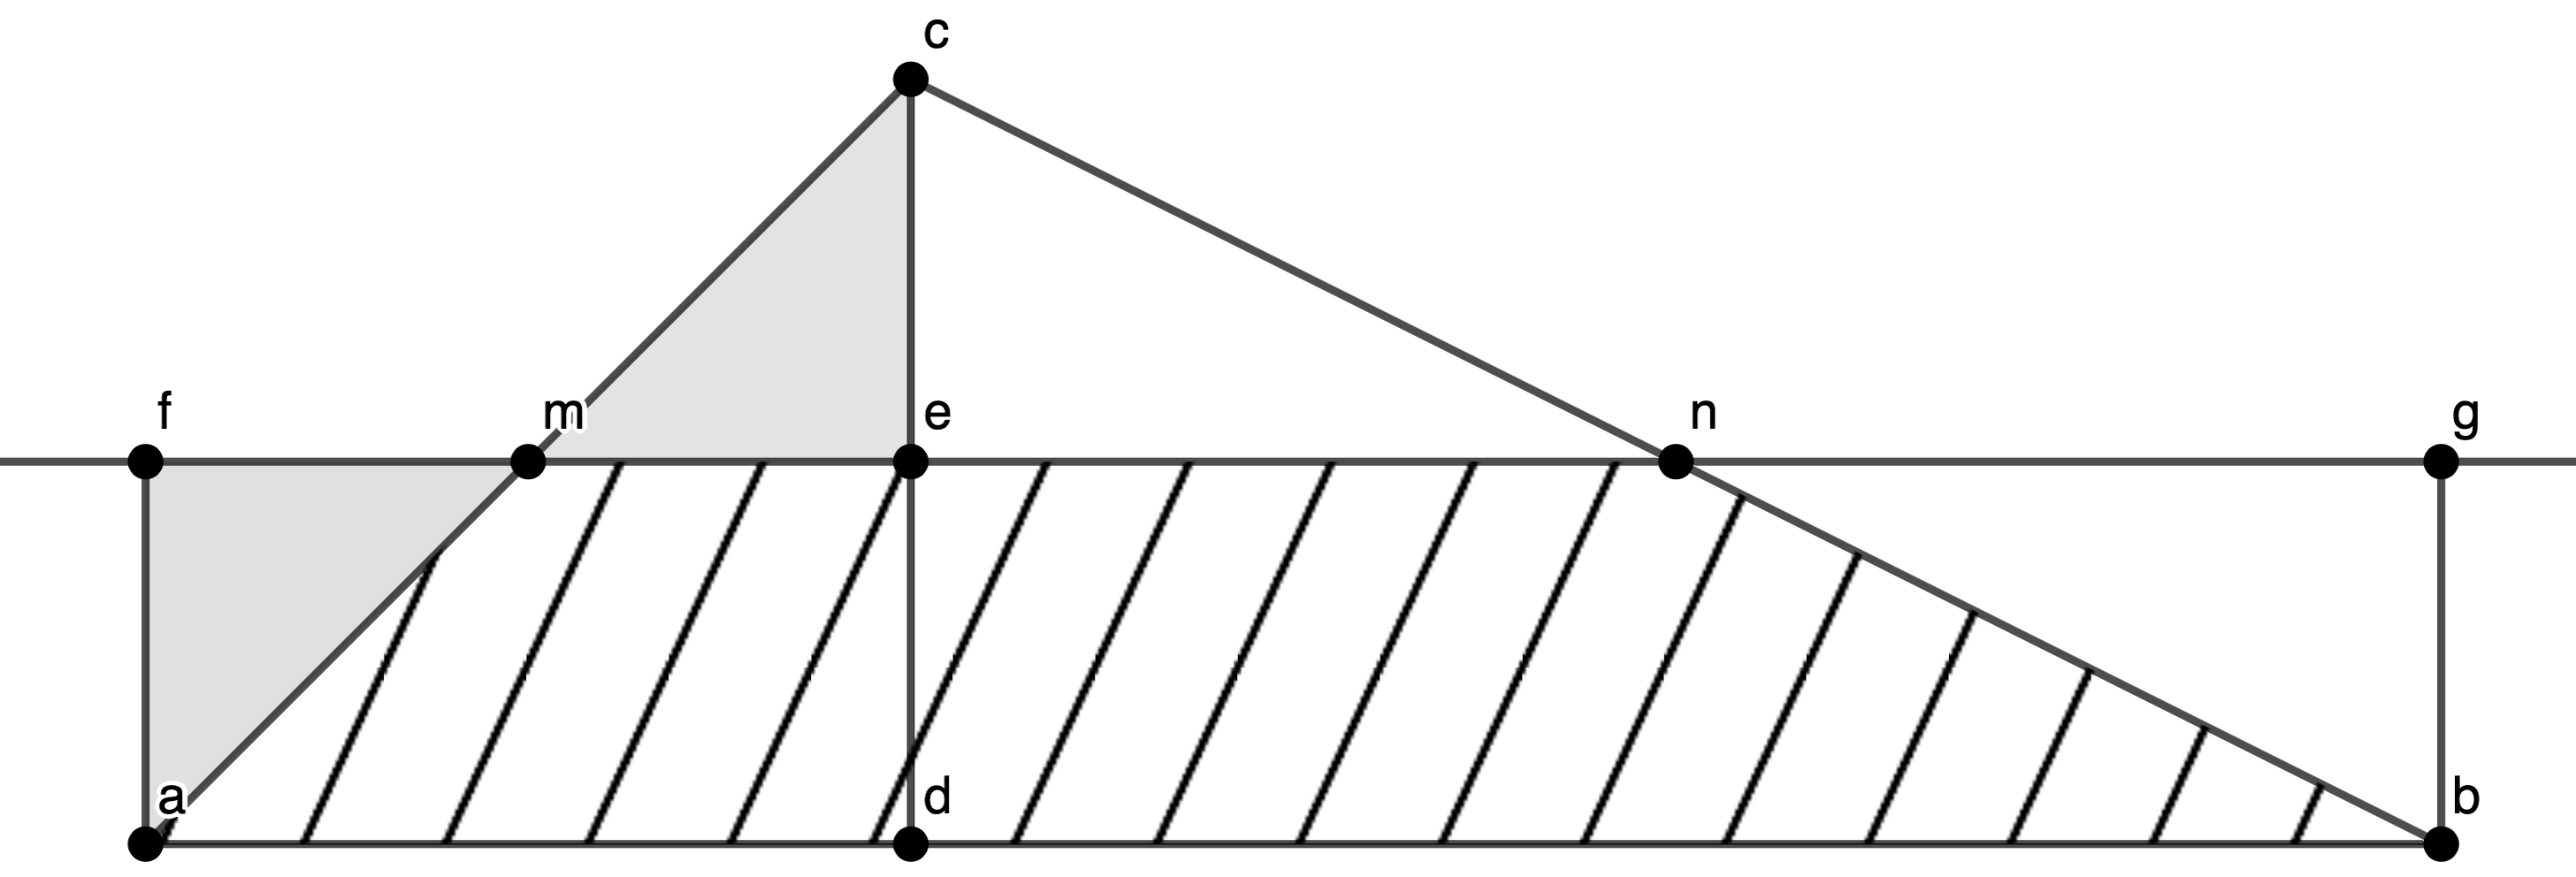
\includegraphics[scale=1.6]{DreieckLemma}
		\caption{Zerlegung eines Dreiecks in ein Rechteck}
		\label{Abb.1}
	\end{figure}
	
	\begin{lemma} \label{lemma:rechtecke}
		Zwei beliebige Rechtecke mit dem gleichen Flächeninhalt sind zerlegungsgleich.
	\end{lemma}
	
	\begin{proof}
		Seien $P$ und $Q$ zwei Rechtecke mit dem gleichen Flächeninhalt, d.~h. falls $h_P$ die Höhe und 
		$b_P$ die Breite des Rechtecks $P$ und $h_Q$ die Höhe und $b_Q$ die Breite des Rechtecks $Q$ sind, 
		dann soll gelten $h_P \cdot b_P = h_Q \cdot b_Q$ also auch
		\begin{align}
			\frac{b_P}{h_Q}=\frac{b_Q}{h_P}. \label{lemma:rechteck;1}
		\end{align}
		\begin{figure}[!htbp]
			\centering
			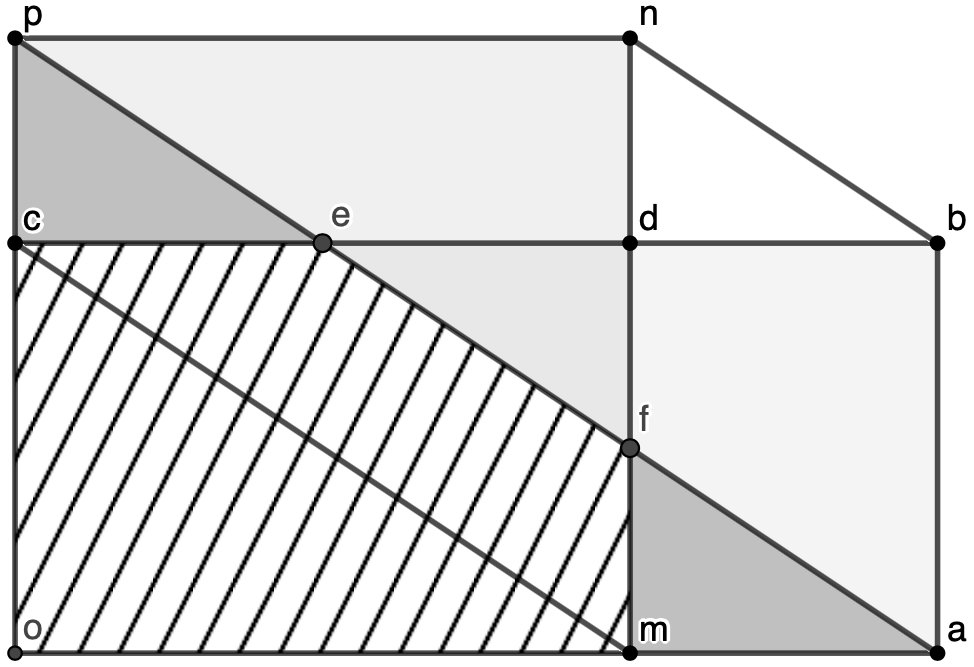
\includegraphics[scale=1.4]{Rechteck}
			\caption{Zerlegung zweier Rechtecke}
			\label{Abb.2}
		\end{figure}
		Seien $o,a,b,c$ die Eckpunkte des Rechtecks $P$ und $o,m,n,p$ die Eckpunkte des Rechtecks $Q$, siehe 
		Abbildung \ref{Abb.2}. 
		Wir verschieben hier $Q$ so auf $P$, dass beide eine gemeinsame Ecke $o$ mit rechtem Winkel haben. 
		Dies ändert nichts am Resultat. 
		Die Höhe $h_P$ soll also der Länge der Strecken $\overline{co}$ und $\overline{ab}$ entsprechen. Die 
		Breite $b_P$ soll der Länge der Strecken $\overline{oa}$ und $\overline{bc}$ entsprechen. Analog soll 
		$h_Q$ der Länge der Strecken $\overline{po}$ und $\overline{mn}$ und $b_Q$ der Länge der Strecken 
		$\overline{om}$ und $\overline{np}$ entsprechen. Wegen Gleichung  \ref{lemma:rechteck;1} sehen wir also, dass 
		die Strecken $\overline{mc}$ und $\overline{ap}$ parallel sind. Außerdem stellen wir fest, dass gilt
		\[ (b_P-b_Q)h_P=b_P h_P-b_Q h_P=h_Qb_Q-b_Qh_P=b_Q(h_Q-h_P) \]
		also auch
		\[\frac{b_P-b_Q}{h_Q-h_P}=\frac{b_Q}{h_P}. \]
		Damit folgt, dass die Dreiecke $omc$ und $dbn$ ähnlich sind, d.~h. 
		sie haben die gleichen Seitenverhältnisse und folglich sind die Strecken $\overline{mc}$ 
		und $\overline{nb}$ parallel. Hierbei sei $d$ der Schnittpunkt der Strecken $\overline{mn}$ und 
		$\overline{bc}$. Also sind die drei Strecken $\overline{mc}$, $\overline{ap}$ und $\overline{nb}$ 
		parallel. Nun unterscheiden wir zwei Fälle
		\begin{enumerate}
			\item \textsl{Fall:} Die Verbindungsstrecke $\overline{ap}$ der Eckpunkte schneidet das 
			Rechteck $omdc$ in den Punkten $e$, mit der Seite $\overline{dc}$, 
			und $f$, mit der Seite $\overline{md}$, siehe Abbildung \ref{Abb.2}. 
			Es gilt $2b_Q\geq b_P$.
			Also sind die beiden in der Abbildung grau hinterlegten Dreiecke $maf$ und $cep$ und die beiden 
			in der Abbildung hellgrau hinterlegten Dreiecke $abe$ und $fnp$ kongruent. Mit dem übrig gebliebenen, 
			in der Abbildung schraffierten Fünfeck $omfec$ ist unsere Zerlegung komplett.
			
			\item \textsl{Fall:} Die Verbindungsstrecke $\overline{ap}$ der Eckpunkte schneidet das 
			Rechteck $omdc$ nicht, siehe Abbildung \ref{Abb.3}. 
			Es gilt also $2b_Q<b_P$. Sei nun $e$ der Mittelpunkt der Strecke $\overline{oa}$. Weiter sei $k$ die 
			kleinste natürliche Zahl, die angibt, wie oft man die Strecke $\overline{om}$ entlang der Strecke $\overline{oa}$ 
			legen muss, s.~d. der äußere Eckpunkt der $k$-ten Verlegung der Strecke 
			$\overline{om}$ nicht mehr auf der Strecke $\overline{oe}$ liegt, 
			sondern auf der Strecke $\overline{ea}$. Diesen Eckpunkt wollen 
			wir $t$ nennen. 
			Nun zerlegen wir das Rechteck $Q$ in $k$ Rechtecke, deren 
			Basis parallel ist zur Strecke $\overline{om}$, die wir nun entlang der neu enstandenen Strecke 
			$\overline{ot}$ legen. Wir erhalten, somit das zu $Q$ zerlegungsgleiche Rechteck $otuv$. 
			Sei die Breite dieses Rechtecks nun $b'$, die die Bedingung
			\[ 2b'>b_P \]
			erfüllt. Damit können wir nach dem ersten Fall sagen, dass die Rechtecke $P$ und $otuv$ 
			zerlegungsgleich sind. Mit der Transitivität der 
			Zerlegungsgleichheit (Proposition \ref{lemma:transitiv}) sind 
			also auch $P$ und $Q$ zerlegungsgleich.
		\end{enumerate}
		Damit sind $P$ und $Q$ zerlegungsgleich.
	\end{proof}
	
	\begin{figure}[!htbp]
		\centering
		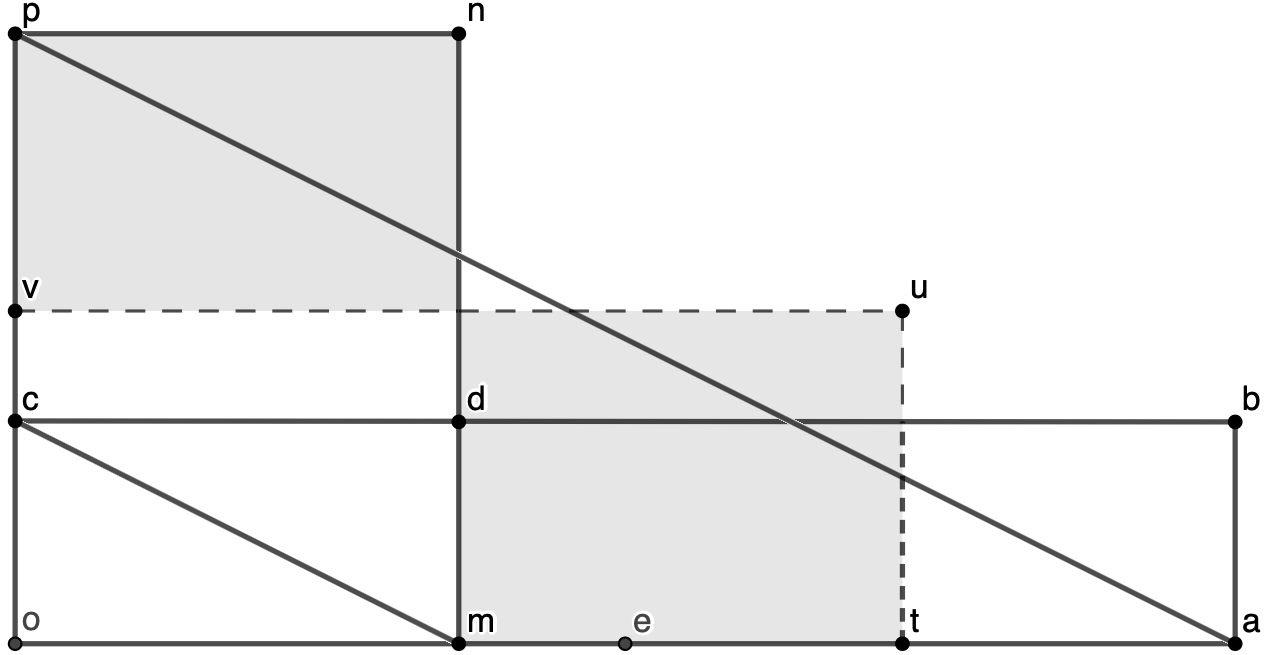
\includegraphics[scale=0.8]{Rechteck2}
		\caption{Zerlegung zweier Rechtecke}
		\label{Abb.3}
	\end{figure}
	
	\begin{theorem}[Bolyai-Gerwien Theorem] \label{theorem:bolyai-gerwien}
		Zwei beliebige Polygone mit dem gleichen Flächeninhalt sind zerlegungsgleich.
	\end{theorem}
	
	\begin{proof}
		Sei $P$ ein Polygon. Dann kann $P$, wie wir später in Satz \ref{thm:simplzerl} sehen werden, in endlich viele disjunkte Dreiecke zerlegt werden und jedes dieser 
		Dreiecke ist nach Lemma \ref{lemma:dreieck,rechteck} zerlegungsgleich zu einem Rechteck. Wir finden 
		also für $P$ die Darstellung
		\[ P\sim P_1+\ldots+P_n,\]
		wobei $P_1,\ldots,P_n$ Rechtecke sind. Nun nehmen wir eine beliebige Kante $\overline{a_0b_0}$ und 
		stellen die Lotgeraden auf den Eckpunkten $a_0$ und $b_0$ durch die Strecke $\overline{a_0b_0}$ 
		auf. Anschließend ziehen wir $n$ 
		parallele Strecken zu $\overline{a_0b_0}$, s.~d. der Flächeninhalt des Recheckts $a_{i-1}b_{i-1}b_ia_i$, 
		welches wir $R_i$ nennen, dem Flächeninhalt des Rechtecks $P_i$ entspricht, wobei $i=1,\ldots,n$. 
		Nach Lemma \ref{lemma:rechtecke} gilt also $P_i\sim R_i$ für alle $i$ und damit
		\[ P_1+\ldots+P_n\sim R_1+\ldots+R_n. \]
		Da $P\sim P_1+\ldots+P_n$ gilt also mit Proposition \ref{lemma:transitiv}
		\[ P\sim R_1+\ldots+R_n\]
		und damit ist $P$ mit dem Rechteck $a_0b_0b_na_n$ zerlegungsgleich. 
		Somit ist jedes Polygon zerlegungsgleich zu einem Rechteck. \\
		Seien nun $P$ und $Q$ zwei Polygone mit gleichem Flächeninhalt, dann finden wir wie bereits oben gezeigt 
		Rechtecke $R_1$ und $R_2$, s.~d.
		\[ P\sim R_1,\quad Q\sim R_2.\]
		Nach Proposition \ref{prop:zerl,vol} haben $R_1$ und $R_2$ also das 
		gleiche Volumen und nach Lemma \ref{lemma:rechtecke} gilt also nun auch 
		$R_1\sim R_2$. Mit der Transitivität 
		der Zerlegungsgleichheit 
		(Proposition \ref{lemma:transitiv}) folgt, dass $P\sim Q$ gilt.
	\end{proof}
	
	Wir haben gesehen, dass sich jedes beliebige Polygon in Dreiecke zerlegen lässt. Diese Dreiecke 
	sind nach Lemma \ref{lemma:dreieck,rechteck} zerlegungsgleich zu Rechtecken mit gleichem 
	Flächeninhalt. Mit Satz \ref{theorem:bolyai-gerwien} können wir die Rechtecke zerlegen in Rechtecke 
	mit gleicher Grundseite. Dieses Verfahren können wir nun auf beliebige Polygone mit gleichem Flächeninhalt 
	anwenden. Da diese Rechtecke nach Lemma \ref{lemma:rechtecke} zerlegungsgleich sind, folgt mit der 
	Transitivität der Zerlegungsgleichheit aus Proposition \ref{lemma:transitiv} die Zerlegungsgleichheit der Polygone. \\
	Wir haben nun den Fall in der Ebene abgeschlossen und können in 
	den dreidimensionalen Raum übergehen. 
	
	\newpage
	
	\section{Zerlegungsgleichheit von Polyedern}
	
	Im Folgenden setzen wir die Dimension $d$ auf $3$, d.~h. wir betrachten Polyeder. 
	
	\begin{definition}
		Wir wollen den Schnitt 
		einer der Hyperebenen, durch die der Polyeder definiert ist, mit dem 
		Polyeder eine \textsl{Seite} des Polyeders nennen. Den Schnitt 
		zweier Seiten nennen wir eine \textsl{Kante} und den Schnitt zweier 
		Kanten eine \textsl{Ecke} des Polyeders.
	\end{definition}
	Max Dehn fand bereits 1901 heraus, 
	dass die Kanten des Polyeders der Teil sind, der beim Zerschneiden 
	eine entscheidende Rolle spielt. Sie sind sozusagen 
	der Knackpunkt. 
	Deshalb müssen wir uns zunächst überlegen, was mit den Kanten eines Polyeders $P$ passiert, wenn wir diesen in zwei 
	Polyeder $P_1$ und $P_2$ zerlegen. 
	\begin{definition}
		Sei $k$ eine Kante des Polyeders $P$.  Wir wollen jeder Kante $k$ ihre \textsl{Länge} $\ell(k)\in\setR_+$ zurodnen, also den größten 
		Abstand zwischen den Punkten der Kante. Weiter ordnen wir $k$ den \textsl{Diederwinkel} $w(k)\in(0,2\pi)$, 
		also den Winkel innerhalb des Polyeders zwischen den beiden Hyperebenen, 
		durch die die Kante $k$ entsteht, zu.
	\end{definition}
	Sei $\ell(k)=l$ die Länge der Kante $k$ und $w(k)=\varphi$ der 
	dazugehörige Diederwinkel. Dann können 
	beim Zerschneiden folgende Fälle eintreten (diese orientieren sich nach 
	den Fällen in \cite{SkriptLA}[7.4]).
	\begin{enumerate}
		\item \label{bem:dehn;1} 
		Wir schneiden durch die Kante: Es entstehen zwei neue Kanten $k_1$ von $P_1$ und $k_2$ von $P_2$, 
		deren Kantenlängen sich zu der von $k$ addieren lassen und deren Winkel gleich dem von $k$ sind. 
		d.~h. für $\ell(k_1)=l_1$ und $\ell(k_2)=l_2$ gilt $l=l_1 +l_2$.
		\item \label{bem:dehn;2} 
		Wir schneiden entlang der Kante: Also entstehen zwei neue Kanten $k_1$ von $P_1$ und $k_2$ von 
		$P_2$, deren Kantenlänge gleich der von $k$ ist und deren Winkel sich zu dem von $k$ addieren lassen. 
		d.~h. für $w(k_1)=\varphi_1$ und $w(k_2)=\varphi_2$ gilt $\varphi=\varphi_1 +\varphi_2$.
		\item \label{bem:dehn;3} 
		Wir schneiden nicht durch die Kante: Die Kante $k$ lässt sich entweder in $P_1$ oder $P_2$ 
		wiederfinden und sowohl Kantenlänge, als auch Diederwinkel bleiben gleich.
		\item \label{bem:dehn;4} 
		Bleibt nur noch der Sonderfall, wenn wir durch eine der Flächen von $P$ schneiden. Hierbei entstehen zwei neue Kanten $k_1$ von $P_1$ und $k_2$ von $P_2$, deren Längen gleich sind und deren Winkel sich zu $\pi$ addieren lassen. d.~h. für $w(k_1)=\varphi_1$ und 
		$w(k_2)=\varphi_2$ gilt $\varphi_1 +\varphi_2 =\pi$.
	\end{enumerate}
	Wir wollen eine Operation, die in beiden Argumenten, sowohl in Länge als auch Diederwinkel, linear ist 
	und bei der wir einen Diederwinkel $\pi$ mit $0$ identifizieren. Dies führt uns auf das Tensorprodukt.
	
	\subsection{Tensoren}
	
	Tensoren sind bereits aus der Linearen Algebra bekannt. Wir wiederholen hier 
	noch einmal ihre universelle Eigenschaft.
	
	\begin{proposition}[Universelle Eigenschaft] \label{prop:univeig}
		Sei $R$ ein kommutativer Ring mit Eins und seien $M$ und $N$ zwei $R$-Moduln. Dann ist das 
		\textsl{Tensorprodukt} $M\otimes_R N$ genau derjenige $R$-Modul, zu dem es eine bilineare Abbildung 
		$\otimes: M\times N \to M\otimes_R N$ gibt, die die folgende universelle Eigenschaft erfüllt:
		\begin{center}
			Sei $L$ ein weiterer $R$-Modul und $\phi: M\times N \to L$ eine bilineare Abbildung. Dann 
			existiert genau eine lineare Abbildung $\eta: M\otimes_R N \to L$, s.~d. das folgende Diagramm 
			kommutiert:
			\begin{center}
				\begin{tikzpicture}
					\node(R1) at (0,0){$M\times N$};
					\node[right = 2 of R1](k){$L$};
					\node[below = 1 of R1](R2){$M\otimes N$};
					
					\draw[->] (R1) -- (k) node[midway,above]{$\phi$};
					\draw[->] (R1) -- (R2) node[midway,left]{$\otimes$};
					\draw[->,dashed] (R2) -- (k) node[midway,below]{$\exists ! \eta$};
				\end{tikzpicture}
			\end{center}
		\end{center}
		Gibt es einen solchen $R$-Modul $M\otimes_R N$, dann ist dieser bis auf Isomorphie eindeutig bestimmt.
	\end{proposition}
	
	\begin{proof}
		Für den Beweis verweise ich auf \cite[Proposition 2.12]{introductiontocomalg} und \cite[Satz 7.3]{SkriptLA}.
	\end{proof}
	
	Demzufolge wissen wir nun, dass das Tensorprodukt folgende Eigenschaften erfüllt: \\ 
	Sei $R$ ein kommutativer Ring 
	mit Eins und $R$-Moduln $M$ und $N$, dann gilt für alle $m,m'\in M$, $n,n'\in N$ und $r,r'\in R$
	\begin{align*}
		(mr+m'r'\otimes n)=(m\otimes n)\cdot r +(m'\otimes n)\cdot r' \\
		(m\otimes nr+n'r')=(m\otimes n)\cdot r+(m\otimes n')\cdot r'.
	\end{align*}
	
	Damit ist der bilineare Operator gefunden. Wir wollen für unser Problem den Spezialfall 
	$\setR \otimes_{\setZ} \setR / \pi\setZ$ betrachen. Hierbei identifizieren wir die Länge einer Kante mit dem 
	ersten Argument und den Winkel einer Kante mit dem zweiten Argument. 
	Den Winkel $\pi$ identifizieren wir in $\setR/\pi\setZ$ mit $0$. Das 
	Tensorprodukt erfüllt also alle gewollten Eigenschaften. 
	
	\subsection{Die Dehn-Invariante}
	
	\begin{definition}[Dehn-Invariante]
		Sei $P$ ein dreidimensionaler beschränkter Polyeder mit den Kanten $k_1,\ldots,k_n$. Dann definieren wir die 
		\textsl{Dehn-Invariante} $D(P)\in \setR \otimes_{\setZ}\setR/\pi \setZ$ durch
		\[ \sum_{i=1}^n \ell(k_i)\otimes [w(k_i)]. \]
	\end{definition}
	
	Wir müssen nun zeigen, dass die Dehn-Invariante sich beim Zerschneiden eines Polyeders nicht 
	verändert und somit eine Invariante ist.
	
	\begin{proposition}[Invarianz] \label{prop:invarianz}
		Sei $P$ ein Polyeder und $P=P_1+P_2$ eine Zerlegung von $P$ in zwei Polyeder $P_1$ und $P_2$, dann 
		gilt $D(P_1+P_2)=D(P_1)+D(P_2)$.	
	\end{proposition}
	
	\begin{proof}
		Sei $P$ ein beschränkter Polyeder, den wir in zwei Polyeder $P_1$ und $P_2$ zerschneiden. 
		Die Summe der  Dehn-Invarianten der einzelnen Polyeder soll gerade der Dehn-Invariante von $P$ 
		entsprechen. Dazu betrachten wir die Kanten der Polyeder und überlegen, was für die Summanden gilt. Es 
		reicht, die Fälle zu betrachten, die wir am Anfang des Kapitels erwähnt haben.
		\begin{itemize}
			\item Zu \ref{bem:dehn;1}: Beim Schneiden durch eine Kante $k$ von $P$ entstehen zwei 
			neue Kanten $k_1$ von $P_1$ und $k_2$ von $P_2$, wobei die Längen sich addieren und die Winkel  
			gleich bleiben. Es gilt
			\[ \ell(k_1)\otimes w(k) + \ell(k_2)\otimes w(k)=(\ell(k_1)+\ell(k_2))\otimes w(k)=
			\ell(k)\otimes w(k).\]
			Also verändert sich die Dehn-Invariante nicht.
			\item Zu \ref{bem:dehn;2}: Beim Schneiden entlang einer Kante $k$ von $P$ entstehen zwei neue Kanten 
			$k_1$ von $P_1$ und $k_2$ von $P_2$, wobei die Längen gleich bleiben und die Winkel sich addieren. 
			Es gilt
			\[ \ell(k)\otimes  w(k_1)+\ell(k)\otimes w(k_2)=\ell(k)\otimes (w(k_1)+w(k_2))=
			\ell(k)\otimes w(k).\]
			Also verändert sich auch hier die Dehn-Invariante nicht.
			\item Zu \ref{bem:dehn;3}: Wir schneiden nicht durch die Kante $k$ von $P$, demnach finden wir die Kante mit gleicher Länge und gleichem 
			Winkel in $P_1$ oder $P_2$ wieder und damit bleibt 
			der Summand und somit die Dehn-Invariante gleich. 
			\item Zu \ref{bem:dehn;4}: Beim Schneiden durch eine Fläche entstehen zwei neue Kanten $k_1$ von 
			$P_1$ und $k_2$ von $P_2$, deren Längen gleich sind und Winkel sich zu $\pi$ addieren lassen. Es gilt 
			\[ \ell(k_1)\otimes w(k_1)+\ell(k_1)\otimes w(k_2)=\ell(k_1)\otimes (w(k_1)+w(k_2))=
			\ell(k_1)\otimes \pi=\ell(k_1)\otimes 0=0. \]
			Also ändert auch dies nichts an der Dehn-Invariante.
		\end{itemize}
		Damit gilt für alle Kanten $k$ von $P$ und alle Kanten $k_1$ von $P_1$ 
		und $k_2$ von $P_2$ also
		\[D(P)=\sum_k \ell(k)\otimes w(k)=\sum_{k_1}\ell(k_1)\otimes w(k_1)+
		\sum_{k_2}\ell(k_2)\otimes w(k_2)=D(P_1)+D(P_2).\]
	\end{proof}
	
	Im Beweis haben wir lediglich die Bilinearität des Tensorprodukts ausgenutzt. 
	Wir können dieses Resultat auf endlich viele Zerlegungen von $P$ fortsetzen. 
		
	\begin{proposition} \label{prop:cong,dehn}
		Seien $P$ und $Q$ zwei Polyeder, s.~d. $P\cong Q$, dann gilt $D(P)=D(Q)$.
	\end{proposition}
	
	\begin{proof}
		Isometrien erhalten sowohl Kantenlängen, als auch Diederwinkel der Polyeder und damit bleibt auch 
		die Dehn-Invariante unverändert.
	\end{proof}
	
	\begin{theorem}[Dehn] \label{thm:dehn}
		Seien $P$ und $Q$ zerlegungsgleiche Polyeder, dann gilt $D(P)=D(Q)$ und $vol(P)=vol(Q)$.
	\end{theorem}
	
	\begin{proof}
		Seien $P=P_1+\ldots+P_n$ und $Q=Q_1+\ldots+Q_n$ die Zerlegungen von $P$ und 
		$Q$, also $P_i\cong Q_i$ für alle $i=1,\ldots,n$. Dann folgt mit Proposition \ref{prop:zerl,vol}
		dass $vol(P)=vol(Q)$. Außerdem gilt mit den Propositionen \ref{prop:cong,dehn}
		und \ref{prop:invarianz}
		\[D(P)=D(P_1+\ldots+P_n)=\sum_{i=1}^n D(P_i) =\sum_{i=1}^n D(Q_i)=D(Q_1+\ldots+Q_n)=D(Q).\]
	\end{proof}
	
	Im Jahr 1965 bewies der Schweizer Mathematiker Jean-Pierre Sydler (in 
	\cite{Sydler1965}) 
	sogar, dass die Zerlegungsgleichheit eine notwendige Bedingung ist und 
	es ergibt sich der folgende Satz. Wir werden diesen hier nicht beweisen.
	
	\begin{theorem}[Dehn-Sydler Theorem]
		Seien $P$ und $Q$ Polyeder, dann sind $P$ und $Q$ genau 
		dann zerlegungsgleich, wenn die Dehn-Invariante und das Volumen 
		der Polyeder gleich sind.
	\end{theorem}
	
	\subsection{Lokalisierung des Tensorprodukts}
	
	Um später die Dehn-Invariante einiger Polyeder berechnen zu können, 
	wollen wir uns ein paar Eigenschaften des Tensorprodukts 
	$\setR\otimes_{\setZ}\setR /\pi\setZ$ anschauen. Dazu wollen wir zeigen, dass unser Tensorprodukt isomorph zum Tensorprodukt  
	$\setR\otimes_{\setQ}\setR /\pi\setQ$ ist, hierzu benötigen wir ein 
	paar Resultate 
	aus der Kommutativen Algebra. Wir richten uns in diesem Abschnitt 
	nach \cite{introductiontocomalg}[Kapitel 3].\\
	Sei im Folgenden $R$ ein Integritätsring, wir wollen in diesem nun 
	Brüche einführen. Sei dazu $S$ eine multiplikative Teilmenge von $R$, d.~h.
	$1\in S$ und $S$ ist unter Multiplikation abgeschlossen, also ein Monoid. Wir 
	definieren die Relation $\equiv$ auf $R\times S$ durch
	\[(r_1,s_1)\equiv(r_2,s_2)\quad \Leftrightarrow\quad r_1 s_2 =r_2 s_1\]
	für Elemente $r_1,r_2\in R$ und $s_1,s_2\in S$. \\
	Wir stellen fest, dass diese Relation  eine Äquivalenzrelation ist. Die 
	Reflexivität und Symmetrie sind klar, wir zeigen also noch die Transitivität.
	Es gelte $(r_1,s_1)\equiv(r_2,s_2)$ und $(r_2,s_2)\equiv(r_3,s_3)$ für 
	$r_1,r_2,r_3\in R$ und $s_1,s_2,s_3\in S$, also gilt $r_1 s_2= r_2 s_1$ und 
	$r_2 s_3 =r_3 s_2$ und damit $r_1 s_2 r_2 s_3 =r_2 s_1 r_3 s_2$. Falls $r_2=0$ 
	oder $s_2=0$ 
	ist klar, dass $(r_1,s_1)\equiv(r_3,s_3)$ gilt, falls $r_2\neq 0$ können wir $r_2$ und $s_2$ aus der Gleichung streichen und es folgt 
	$r_1 s_3=r_3 s_1$ und damit $(r_1,s_1)\equiv(r_3,s_3)$. \\
	Wir schreiben $\frac{r}{s}$ für die Äquivalenzklasse 
	von $(r,s)$ und $S^{-1}R$ 
	für die Menge aller Äquivalenzklassen. 
	Wir können $S^{-1}R$ nun eine Ringstruktur geben, indem wir die Addition und Multiplikation für 
	alle $r_1,r_2\in R$ und $s_1,s_2\in S$ definieren durch
	\begin{align*}
		\left(\frac{r_1}{s_1}\right)+\left(\frac{r_2}{s_2}\right)
		&=\left(\frac{r_1s_2+r_2s_1}{s_1s_2}\right) \\
		\left(\frac{r_1}{s_2}\right)\cdot\left(\frac{r_2}{s_2}\right)
		&=\left(\frac{r_1r_2}{s_1s_2}\right).
	\end{align*}
	Wir stellen fest, dass 
	$S^{-1}R$ sogar ein kommutativer Ring mit Eins ist. Außerdem ist 
	$S^{-1}R$ gerade der Quotientenkörper von $R$, falls $S=R\setminus\{0\}$ ist. Betrachten wir beispielweise den Ring 
	$\setZ$ mit der multiplikativen Teilmenge $S=\setZ\setminus\{0\}$, so 
	ist $S^{-1}\setZ$ gerade der Quotientenkörper von $\setZ$, also 
	$\setQ$. Wir können diese Konstruktion nun auch auf Moduln fortführen. 
	Haben wir ein $R$-Modul $M$, dann definieren wir 
	die Äquivalenzrelation wie oben, nur auf $M$, und erhalten die 
	Äquivalenzklassen $\frac{m}{s}$ für Elemente $m\in M$ und $s\in S$. 
	Dann ist $S^{-1}M$ gerade die Menge solcher Brüche und wir erhalten 
	mit $S^{-1}M$ einen $S^{-1}R$-Modul mit der natürlichen Definition 
	der Addition und skalaren Multiplikation. Haben wir nun einen 
	$R$-Modulhomomorphismus $f:M\to N$, dann führt uns dies zu einem 
	$S^{-1}R$-Modulhomomorphismus $S^{-1}f:S^{-1}M\to S^{-1}N$, indem $S^{-1}f$ 
	Elemente $\frac{m}{s}$ aus $S^{-1}M$ auf Elemente $\frac{f(m)}{s}$ 
	aus $S^{-1}N$ abbildet. Für Modulhomomorphismen $f$ und $g$ gilt also 
	\[S^{-1}(f\circ g)=(S^{-1}f)\circ(S^{-1}g).\]
	
	\begin{lemma} \label{lemma:Buch;exakt}
		Sei $R$ ein Integritätsring und $M,M_1,M_2$ seien $R$-Moduln. Weiter 
		sei die Sequenz
		\begin{align}
			M_1\xrightarrow{f}M\xrightarrow{g}M_2 \label{lemma:exakt;1}
		\end{align}
		exakt\footnote{Zur Erinnerung: Eine Sequenz $M_1\xrightarrow{f}M\xrightarrow{g}M_2$ ist exakt in $M$, falls 
			$im(f)=ker(g)$.} in $M$. Dann ist die Sequenz
		\[S^{-1}M_1 \xrightarrow{S^{-1}f}S^{-1}M\xrightarrow{S^{-1}g}S^{-1}M_2\]
		exakt in $S^{-1}M$.
	\end{lemma}
	
	Siehe dazu auch \cite[Proposition 3.3]{introductiontocomalg}.
	
	\begin{proof}
		Sei $m_1\in M_1$ dann gilt $f(m_1)\in im(f)=ker(g)$, wegen der Exaktheit 
		von \ref{lemma:exakt;1} in $M$ und damit ist $g(f(m_1))=0$. Also gilt 
		$g\circ f=0$ und damit erhalten wir
		\[(S^{-1}g) \circ (S^{-1}f) = S^{-1}(g\circ f)=S^{-1}(0)=0.\]
		Demzufolge gilt
		\[im(S^{-1}f)\subset ker(S^{-1}g).\]
		Um die umgekehrte Inklusion zu zeigen, wählen wir 
		$\frac{m}{s}\in ker(S^{-1}g)$, das heißt $S^{-1}g\left(\frac{m}{s}\right)=\frac{g(m)}{s}=0$ in $S^{-1}M_2$. 
		Das wiederum bedeutet, dass $g(m)=0$ in $M_2$, da $R$ ein Integritätsring 
		ist, also auch $m\in ker(g)=im(f)$, wegen der Exaktheit von $M$ in 
		\ref{lemma:exakt;1}. Demnach gibt es ein $m_1\in M_1$ mit $f(m_1)=m$ und damit 
		gilt
		\[\frac{m}{s}=\frac{f(m_1)}{s}=(S^{-1}f)\left(\frac{m_1}{s}\right)\in im(S^{-1}f).\]
		Es folgt 
		\[ker(S^{-1}g)\subset im(S^{-1}f).\]
	\end{proof}

	Nun zurück zu unserem Problem. Wir wollen wissen, was passiert, wenn 
	wir in dem $\setZ$-Modul $\setR /\pi\setZ$ Brüche einführen. Um das 
	zu verstehen, hilft uns das folgende Resultat.
	
	\begin{lemma}
		Sei $M$ ein $R$-Modul und $N$ ein $R$-Untermodul von $M$. Dann sind die $S^{-1}R$-Moduln $S^{-1}(M/N)$ und 
		$S^{-1}M/S^{-1}N$ isomorph.
	\end{lemma}
	
	Siehe \cite[Korollar 3.4 (iii)]{introductiontocomalg}.
	
	\begin{proof}
		Wir betrachten hierzu die Sequenz
		\[0\to N\xrightarrow{f} M\xrightarrow{g} M/N\xrightarrow{h} 0,\]
		wobei $f,g$ und $h$ hier Modulhomomorphismen sind. Die Funktion 
		$f$ bettet das Untermodul $N$ in $M$ ein, also gilt 
		$im(f)=N$. Weiter bildet die Funktion $g$ gerade die Elemente aus $M$ 
		auf deren Äquivalenzklassen in $M/N$ ab und da für alle $n\in N\subset M$ 
		gilt, dass $g(n)=[n]=0$ in $M/N$, folgt auch, dass $ker(g)=N$. Damit 
		ist die Sequenz in $M$ exakt. \\
		Weiter ist $im(g)=M/N$ und da $h$ die Nullabbildung ist, gilt $ker(h)=M/N$. 
		Somit ist die Sequenz auch in $M/N$ exakt. \\
		Wir wenden $S^{-1}$ auf die Sequenz an, dann ist die Sequenz
		\begin{align}
			0\to S^{-1}N \xrightarrow{S^{-1}f} S^{-1}M \xrightarrow{S^{-1}g}
			S^{-1}(M/N)\to 0 \label{lemma:Brüche;1}
		\end{align}
		mit Lemma \ref{lemma:Buch;exakt} in $S^{-1}M$ und $S^{-1}(M/N)$ exakt. \\
		Wir wollen den Homomorphiesatz\footnote{Für einen Modulhomomorphismus 
		$f:M\to N$, induziert der Homomorphiesatz einen Isomorphismus 
		$g:M/ker(f)\to im(f)$.} auf den Modulhomomorphismus 
		$S^{-1}g$ anwenden und erhalten mit der Exaktheit von \ref{lemma:Brüche;1} 
		in $S^{-1}M$
		\[ S^{-1}(M/N)=im(S^{-1}g)\simeq S^{-1}M/ker(S^{-1}g) =S^{-1}M/im(S^{-1}f)=S^{-1}M/S^{-1}N.\]
	\end{proof}
	
	Wenden wir das nun auf das $\setZ$-Modul $\setR /\pi\setZ$ mit 
	$S=\setZ\setminus\{0\}$ an, dann sind die $(\setZ\setminus\{0\})^{-1}\setZ$- also $\setQ$-Moduln 
	$(\setZ\setminus\{0\})^{-1}(\setR /\pi\setZ)$ und 
	$\left((\setZ\setminus\{0\})^{-1}\setR\right) /\left((\setZ\setminus\{0\})^{-1}\pi\setZ\right)$ 
	isomorph. Wir bemerken, dass $(\setZ\setminus\{0\})^{-1}\setR\simeq\setR$ und 
	$(\setZ\setminus\{0\})^{-1}\pi\setZ\simeq\pi\setQ$. Damit gilt also 
	\[ (\setZ\setminus\{0\})^{-1}(\setR /\pi\setZ)\cong \setR/\pi\setQ.\]
	
	\begin{lemma} \label{lemma:lociso}
		Sei $R$ ein Integritätsring und $M$ ein $R$-Modul. Dann gibt es einen 
		eindeutigen Isomorphismus
		\[f:S^{-1}R\otimes_R M\to S^{-1}M\]
		zwischen den $S^{-1}R$-Moduln, s.~d.
		\begin{align}
			f\left(\frac{r}{s}\otimes m\right)=\frac{rm}{s} \label{lemma:lociso;1}
		\end{align}
		für alle $r\in R$, $m\in M$ und $s\in S$.
	\end{lemma}
	
	Der Beweis richtet sich nach \cite[Proposition 3.5]{introductiontocomalg}.
	
	\begin{proof}
		Die Abbildung $g:S^{-1}R\times M\to S^{-1}M$ mit $g\left(\frac{r}{s},m\right)=\frac{rm}{s}$ ist bilinear, da 
		\begin{align*}
			&g\left(\lambda_1\left(\frac{r_1}{s_1}+\frac{r_2}{s_2}\right),
			\lambda_2 (m_1+m_2)\right)=g\left(\frac{\lambda_1 (r_1 s_2+r_2
			 s_1)}{s_1s_2},\lambda_2(m_1+m_2)\right) \\
			&=\frac{\lambda_1(r_1s_2+r_2s_1)\lambda_2(m_1+m_2)}{s_1s_2}\\
			&=\lambda_1\lambda_2\left(\frac{r_1(m_1+m_2)}{s_1}+
			\frac{r_2(m_1+m_2)}{s_2}\right) \\
			&=\lambda_1\lambda_2 \left(g\left(\frac{r_1}{s_1},m_1\right)
			+g\left(\frac{r_1}{s_1},m_2\right)+g\left(\frac{r_2}{s_2},m_1\right)+
			g\left(\frac{r_2}{s_2},m_1\right)\right)
		\end{align*}
		für alle $r_1,r_2,\lambda_1,\lambda_2\in R$, $s_1,s_2 \in S$ und 
		$m_1,m_2\in M$ gilt. Damit gibt es mit der universellen Eigenschaft 
		des Tensorprodukts (Proposition \ref{prop:univeig}) genau einen 
		$R$-Modulhomomorphismus $f:S^{-1}R\otimes_R M\to S^{-1}M$, s.~d. 
		\ref{lemma:lociso;1} gilt. Es ist klar, dass $f$ surjektiv ist, 
		dazu wählen wir $r=1$ und erhalten somit alle Elemente aus 
		$S^{-1}M$. Weiter ist $f$ auch eindeutig bestimmt durch 
		\ref{lemma:lociso;1}. \\
		Wir zeigen also noch die Injektivität. Dazu betrachten wir die 
		Elemente von $S^{-1}R\otimes_R M$. Sei  
		\[\sum_{i=1}^n \frac{r_i}{s_i}\otimes m_i \in S^{-1}R\otimes_R M\]
		ein beliebiges Element, dann definieren wir
		\[s:=\prod_{i=1}^n s_i\in S,\qquad t_i:=\prod_{\genfrac{}{}{0pt}{1}{j=1}{j\neq i}}^n s_j\in S\]
		und es gilt 
		\[\sum_{i=1}^n \frac{r_i}{s_i}\otimes m_i =
		\sum_{i=1}^n \frac{r_it_i}{s}\otimes m_i =\sum_{i=1}^n 
		\frac{1}{s}\otimes r_i t_i m_i =\frac{1}{s}\otimes\sum_{i=1}^n
		\underbrace{r_it_im_i}_{\in M}.\]
		Wir können demnach jedes Element aus $S^{-1}R\otimes_R M$ in der Form 
		\[\frac{1}{s}\otimes m\]
		schreiben. Betrachten wir nun den Kern von $f$. Sei also 
		$\frac{1}{s}\otimes m \in ker(f)\subset S^{-1}R\otimes_R M$, d.~h. 
		$f\left(\frac{1}{s}\otimes m\right)=0$. Da $R$ ein 
		Integritätsring ist, folgt mit $f\left(\frac{1}{s}\otimes m\right)=\frac{m}{s}=0$, dass $m=0$ und damit gilt
		\[\frac{1}{s}\otimes m =\frac{1}{s}\otimes 0=0.\]
		Damit ist $f$ bijektiv, ergo der gesuchte Isomorphismus.
	\end{proof}
	
	Es lässt sich nun folgendes Resultat zeigen, siehe dazu auch \cite{introductiontocomalg}[Proposition 3.7].
	
	\begin{proposition}\label{prop:tensoriso}
		Seien $M$ und $N$ zwei $R$-Moduln, dann gibt es einen eindeutigen 
		Isomorphismus 
		\[f:S^{-1}M\otimes_{S^{-1}R}S^{-1}N\to S^{-1}(M\otimes_R N)\]
		zwischen den $S^{-1}R$-Moduln, s.~d.
		\[f\left(\frac{m}{s_1}\otimes\frac{n}{s_2}\right)=\frac{m\otimes n}{s_1s_2}.\]
	\end{proposition}

	\begin{proof}
		Es gilt mit Lemma \ref{lemma:lociso} und den kanonischen Isomorphismen des 
		Tensorprodukts
		\begin{align*}
			S^{-1}M\otimes_{S^{-1}R}S^{-1}N &\overset{\ref{lemma:lociso}}{\simeq}
			(S^{-1}R\otimes_R M)\otimes_{S^{-1}R}(S^{-1}R\otimes_R N) \\
			&\overset{\footnotemark}{=}
			 M\otimes_R (\underbrace{S^{-1}R\otimes_{S^{-1}R} S^{-1}R}_{\simeq S^{-1}R})\otimes_R N \\
			&\simeq M\otimes_R S^{-1}R \otimes_R N \\
			&= S^{-1}R \otimes_R(M\otimes_R N) \\
			&\overset{\ref{lemma:lociso}}{\simeq} S^{-1}(M\otimes_R N).
		\end{align*}
	\end{proof}

	\footnotetext{Wir können hier trotz der unterschiedlichen 
		Tensorprodukte die Klammern vertauschen. Siehe dazu auch 
		\cite[Formula 10]{Matsurama}}
	
	Dies lässt sich nun auf unser Tensorprodukt 
	$\setR\otimes_{\setZ}\setR /\pi\setZ$ anwenden, indem wir $R=\setZ$, $M=\setR$ und $N=\setR /\pi\setZ$ setzen und mit 
	$S=\setZ\setminus\{0\}$ und dem obigen Resultat, ergibt sich 
	dann
	\begin{align*}
		S^{-1}R\simeq\setQ,\qquad S^{-1}M\simeq\setR
		\quad\text{ und }\quad S^{-1}N\simeq\setR /\pi\setQ.
	\end{align*}
	Weiterhin gilt
	\[S^{-1}(M\otimes_R N)=(\setZ\setminus\{0\})^{-1}(\setR\otimes_{\setZ}\setR/\pi\setZ)\simeq \setR\otimes_\setZ\setR/\pi\setZ,\]
	denn mit der Bilinearität des Tensorproduktes gilt
	\begin{align*}
		(\setZ\setminus\{0\})^{-1}(\setR\otimes_{\setZ}\setR /\pi\setZ)&\simeq
		\left.\left\langle \left\{\frac{m\otimes n}{z}\right\vert
		 m\in\setR,n\in\setR/\pi\setZ,z\in\setZ\setminus\{0\}\right\}\right\rangle \\
		 &\simeq \left.\left\langle \left\{\frac{m}{z}\otimes n\right\vert m\in\setR,n\in\setR/\pi\setZ,z\in\setZ\setminus\{0\}\right\}
		 \right\rangle \\
		 &\simeq (\setZ\setminus\{0\})^{-1}\setR\ \ \otimes_\setZ\  \setR/\pi\setZ \\
		 &\simeq \setR\otimes_\setZ \setR/\pi\setZ,
	\end{align*}
	wobei wir hier mit $\langle\ \cdot\ \rangle$ das Erzeugnis meinen.
	Insgesamt erhalten wir mit Proposition \ref{prop:tensoriso}
	\begin{align*}
		\setR\otimes_\setZ\setR/\pi\setZ\simeq S^{-1}(M\otimes_R N)\simeq S^{-1}M\otimes_{S^{-1}R}S^{-1}N\simeq\setR\otimes_\setQ\setR/\pi\setQ.
	\end{align*}
	Also gilt
	\begin{align}
		\setR\otimes_\setZ\setR/\pi\setZ\simeq\setR\otimes_\setQ\setR/\pi\setQ. \label{tensor=0}
	\end{align}
	Wir können die Dehn-Invariante auch auf dem $\setQ$-Vektorraum 
	$\setR\otimes_\setQ\setR/\pi\setQ$ betrachten, was uns zu der folgenden 
	Tatsache führt.
	
	\begin{theorem} \label{bem:dehn=0}
		Seien $x\in \setR$ und $y\in\setR/\pi\setQ$ Elemente, dann gilt
		\[ x\otimes y =0 \quad \Leftrightarrow \quad x=0 \ \lor\ y\in\pi\setQ.\]
	\end{theorem}
	
	\begin{proof}
		Die Rückrichtung ist schnell gezeigt, 
		denn für $x\in\setR$ mit $x\neq 0$ und $y=\pi\frac{p}{q}\in\setQ$, wobei $p\in\setZ$ und $q\in\setN$, gilt
		\[ x\otimes y =x\otimes\pi \frac{p}{q} =xp\otimes\frac{\pi}{q} =q\frac{xp}{q}
		\otimes\frac{\pi}{q} = \frac{xp}{q}\otimes\pi =\frac{xp}{q}\otimes 0=0.\]
		Dabei haben wir $p$ zuerst nach links und danach $q$ nach rechts bewegt. \\
		Zur Hinrichtung: Betrachte $\pi\setQ$ ist $1$-dimensionaler 
		$\setQ$-Vektorraum mit Basis $\{\pi\}$ und $\pi\setQ\subset\setR$ ist 
		als $\setQ$-Vektorraum ein 
		Untervektorraum von $\setR$. Wir können also nun 
		unsere Basis mit dem Lemma von Zorn auf ganz $\setR$ fortsetzen. 
		Also hat $\setR$ als $\setQ$-Vektorraum die Basis
		\[\{\pi\}\dot\bigcup B,\]
		wobei $B$ die Menge ist, mit der wir $\{\pi\}$ zu einer Basis von $\setR$ 
		ergänzen. Weiterhin gilt auch
		\begin{align*}
			\setR&\simeq\pi\setQ\oplus\bigoplus_{b\in B}b\setQ\qquad\text{und}\\
			\setR /\pi\setQ&\simeq\qquad\ \ \bigoplus_{b\in B}b\setQ.
		\end{align*}
		Damit ist
		\[\left\{(b_1\otimes b_2)\left\vert b_1\in\pi\setQ\oplus\bigoplus_{b\in B}b\setQ,\ b_2\in \bigoplus_{b\in B}b\setQ\right\}\right.\]
		eine Basis von $\setR\otimes_\setQ\setR/\pi\setQ$. \\
		Zwei Elemente $x\in\setR$ und $y\in\setR/\pi\setQ$ haben demnach die 
		Darstellung
		\begin{align*}
			x&=\alpha\pi+\sum_{b\in B}\beta_b b \\
			y&= \qquad\ \sum_{b'\in B}\gamma_{b'}b',
		\end{align*}
		wobei $\alpha,\beta_b,\gamma_{b'}\in\setQ$ für alle $b,b'\in B$ sind. 
		Falls nun $x\otimes y=0$ gilt also
		\[0=x\otimes y=\left(\alpha\pi+\sum_{b\in B}\beta_b b\right)\otimes
		\left(\sum_{b'\in B}\gamma_{b'}b'\right)=\sum_{b'\in 
		B}\alpha\gamma_{b'}(\pi\otimes b')+\sum_{\genfrac{}{}{0pt}{1}{b\in B}
		{b'\in B}} \beta_b\gamma_{b'}(b\otimes b').\]
		Da $(\pi\otimes b')$ und $(b\otimes b')$ linear unabhängig sind für alle  
		$b,b'\in B$ folgt
		\[\alpha\gamma_{b'}=0\qquad\text{und}\qquad \beta_b\gamma_{b'}=0\]
		für alle $b,b'\in B$. 
		\begin{enumerate}
			\item Falls $\alpha\neq 0$, dann sind $\gamma_{b'}=0$ für alle 
			$b'\in B$ und damit ist $y=0$, also $y\in \pi\setQ$.
			\item Falls $\alpha=0$, dann sind die $\gamma_{b'}$ beliebig. 
			Angenommen es gibt also ein $b\in B$, s.~d. $\beta_b \neq 0$, dann 
			muss $\gamma_{b'}=0$ für alle $b'\in B$ damit $\beta_b\gamma_{b'}=0$ 
			für alle $b'\in B$ gilt. Das wiederum bedeutet $y=0$ und wir sind hier 
			fertig. Falls $\beta_b=0$ für alle $b\in B$, folgt mit $\alpha=0$, 
			dass $x=0$ ist.
		\end{enumerate}
		Damit ist die Aussage bewiesen.
	\end{proof}

	Wir bemerken, dass wir für die Hinrichtung das Auswahl-Axiom 
	benutzt haben. Jedoch ist klar, dass wir bei einer konkreten Berechnung der 
	Dehn-Invariante nur endlich viele Polyeder haben, diese somit auch 
	nur einen endlich-dimensionalen $\setQ$-Untervektorraum von $\setR$ aufspannen und wir somit nicht auf das Auswahl-Axiom angewiesen sind.
	
	Wir erhalten folglich auch:
	
	\begin{corollary}
		Seien $x\in\setR$ und $y\in\setR/\pi\setQ$ Elemente, dann gilt
		\[ x\otimes y\neq0\quad\Leftrightarrow\quad x\neq 0 \ \land\ y\notin\pi\setQ. \]
	\end{corollary}
	
	Folglich ist die Dehn-Invariante eines Polyeders $0$, falls dessen Diederwinkel alle in $\pi\setQ$ liegen. \\
	
	Wir können nun die Dehn-Invarianten einiger Polyeder berechnen.
	
	\subsection{Dehns Lösung}
	
	\begin{example}[Quader] \label{exp:quader}
		Sei $P$ ein dreidimensionaler Quader. Dann gilt für alle Kanten $k$ von $P$, dass $w(k)=\frac{\pi}{2}$. 
		Also gilt $w(k)\in \pi\setQ$ für alle Kanten $k$ und mit Bemerkung \ref{bem:dehn=0} folgt
		\[ D(P)=0. \]
	\end{example}
	
	\begin{example}[regulärer Tetraeder] \label{exp:regTetr}
		Sei $P$ ein dreidimensionaler regulärer Tetraeder, d.~h. alle 
		Kanten von $P$ haben die gleiche Länge $l$ und 
		den gleichen Diederwinkel $\alpha$. Seien $A,B,C,D$ die Ecken von $P$ wie in Abbildung \ref{Abb.4}. 
		Sei $F$ der Mittelpunkt der Strecke $\overline{BC}$, also $|BF|=\frac{l}{2}$ und damit ist nach dem Satz von Pythagoras 
		$|AF|=\frac{\sqrt{3}}{2}l=|DF|$. Der Mittelpunkt $E$ des Dreiecks $ABC$ hat gerade den Abstand 
		$\frac{\sqrt{3}}{3 \cdot 2}l=\frac{l}{2\sqrt{3}}$ zu $F$ und schließlich gilt mit dem Satz von Pythagoras
		\[\cos(\alpha)=\frac{\frac{l}{2\sqrt{3}}}{\frac{\sqrt{3}}{2}l}=\frac{1}{3}\quad\text{also}
		\quad \alpha=\arccos\left(\frac{1}{3}\right). \]
		Damit können wir die Dehn-Invariante berechnen. Es gibt sechs Kanten der Länge $l$, die alle den 
		Diederwinkel $\arccos\left(\frac{1}{3}\right)$ haben, also
		\[ D(P)=\sum_{i=1}^6 l\otimes_{\setZ}\arccos\left(\frac{1}{3}\right)=6l\otimes_{\setZ}\arccos\left(\frac{1}{3}\right).\]
	\end{example}
	
	Siehe auch Beispiel 1 \cite{Proofsfromthebook}.
	
	\begin{figure}[!htbp]
		\centering
		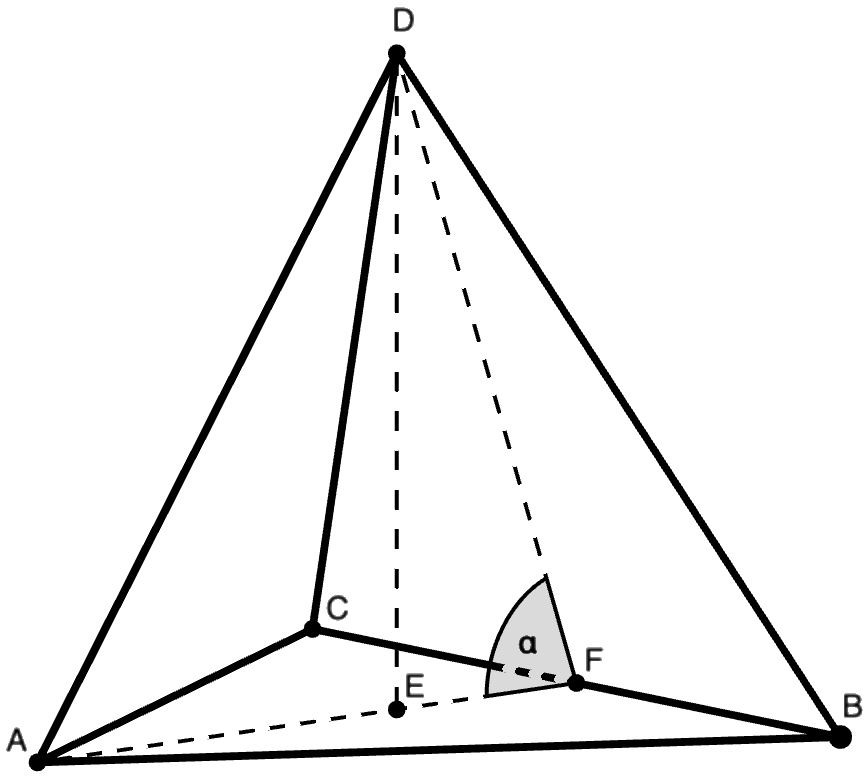
\includegraphics[scale=0.2]{RegulTetraeder}
		\caption{Ein regulärer Tetraeder}
		\label{Abb.4}
	\end{figure}
	
	\begin{proposition} \label{prop:irr}
		Für alle ungeraden $n\in\setN$ mit $n\geq 3$ gilt, dass  $\frac{1}{\pi}\arccos\left(\frac{1}{\sqrt{n}}\right)$ irrational ist.
	\end{proposition}
	
	Wir richten uns hierbei nach \cite{Proofsfromthebook}[Satz 3, Kapitel 8].
	
	\begin{proof}
		Zuerst stellen wir fest, dass mit dem Additionstheorem
		\[\cos(\alpha)+\cos(\beta)=2\cos\left(\frac{\alpha+\beta}{2}\right)\cos\left(\frac{\alpha-\beta}{2}\right) \]
		für $\alpha=(k+1)\varphi$ und $\beta=(k-1)\varphi$ gilt
		\begin{align*}
			\cos\left((k+1)\varphi\right)+\cos\left((k-1)\varphi\right)=&2\cos\left(\frac{(k+1)\varphi+(k-1)\varphi}{2}\right)
			\cos\left(\frac{(k+1)\varphi-(k-1)\varphi}{2}\right) \\
			=& 2\cos(k\varphi)\cos(\varphi)
		\end{align*}
		und damit folgt
		\begin{align}
			\cos((k+1)\varphi)=2\cos(k\varphi)\cos(\varphi)-\cos((k-1)\varphi). \label{prop:irr;1}
		\end{align}
		Wir definieren nun $\varphi_n=\arccos(\frac{1}{\sqrt{n}})$ für $n=2l+1$ mit $l\in\setN$. Dann ist 
		$\cos(\varphi_n)=\frac{1}{\sqrt{n}}$ und $0\leq\varphi_n\leq\pi$. \\
		Mit Induktion über $k\in\setN_0$ zeigen wir, dass gilt
		\begin{align}
			\cos(k\varphi_n)=\frac{A_k}{\sqrt{n}^k}, \label{prop:irr;2}
		\end{align}
		wobei $A_k$ eine ganze Zahl ist, die nicht durch $n$ teilbar ist. Wir beginnen und stellen fest, dass
		\begin{align*}
			&\text{für $k=0$}\qquad 1=\cos(0\cdot\varphi_n)=\frac{A_0}{\sqrt{n}^0}=A_0 \\
			&\text{für $k=1$}\qquad \frac{1}{\sqrt{n}}=\cos({1\cdot\varphi_n})=\frac{A_1}{\sqrt{n}^1}=\frac{A_0}{\sqrt{n}}
		\end{align*}
		und damit $A_0=A_1=1$ ist. Weiterhin gilt mit \ref{prop:irr;1}
		\begin{align*}
			\cos((k+1)\varphi_n)=& 2\cos(k\varphi_n)\cos(\varphi_n) -\cos((k-1)\varphi_n) \\
			=&2\frac{A_k}{\sqrt{n}^k}\cdot\frac{1}{\sqrt{n}}-\frac{A_{k-1}}{\sqrt{n}^{k-1}} \\
			=&\frac{\overbrace{2 A_k-nA_{k-1}}^{=:A_{k+1}}}{\sqrt{n}^{k+1}}.
		\end{align*}
		Da $A_k$ nicht durch $n$ teilbar ist und $n\geq 3$ ungerade, ist die Zahl $2A_k$ auch nicht durch $n$ teilbar 
		und damit auch nicht $A_{k+1}:=2 A_k -nA_{k-1}$. Wir haben also eine konkrete Darstellung für $A_{k+1}$ 
		gefunden und sind mit der Induktion fertig. \\
		Nun kommen wir zum eigentlichen Beweis. Angenommen $\frac{1}{\pi}\varphi_n$ ist 
		rational mit
		\[\frac{1}{\pi}\varphi_n=\frac{m}{k}\]
		für $m\in\setZ$ und $k\in\setN$. Dann gilt mit $k\varphi_n=m\pi$ und \ref{prop:irr;2}
		\[\pm 1=\cos(m\pi)=\cos(k\varphi_n)=\frac{A_k}{\sqrt{n}^k}. \]
		Also auch $\sqrt{n}^k=\pm A_k$. Da $A_k$ eine ganze Zahl ist, ist $\sqrt{n}^k$ auch eine ganze Zahl und somit 
		$k\geq 2$. Damit ist jedoch $n$ ein Teiler von $\sqrt{n}^k$ und da $\sqrt{n}^k \vert A_k$, teilt $n$ auch 
		$A_k$, was ein Widerspruch ist.
	\end{proof}
	
	Damit folgt für $n=9$, dass $\arccos\left(\frac{1}{3}\right)$ nicht in $\pi\setQ$ liegt. Wir erhalten unser 
	folgendes Resultat.
	
	\begin{corollary}[Dehns Lösung]
		Sei $Q$ ein Quader und $T$ ein regulärer Tetraeder mit Kantenlänge $l$. Angenommen 
		$Q$ und $T$ sind zerlegungsgleich, dann gilt mit Satz \ref{thm:dehn} sowohl $vol(Q)=vol(T)$, als auch 
		$D(Q)=D(T)$. 
		Nach Beispiel \ref{exp:quader} gilt $D(Q)=0$ und nach Beispiel \ref{exp:regTetr} gilt
		\[D(T)=6l\otimes_{\setZ}\arccos\left(\frac{1}{3}\right).\]
		Da nach Proposition \ref{prop:irr} $\frac{1}{\pi}\arccos\left(\frac{1}{3}\right)$ irrational ist, liegt
		$\arccos\left(\frac{1}{3}\right)$ nicht in $\pi\setQ$ und damit ist nach Bemerkung \ref{bem:dehn=0} 
		mit $l\neq 0$ auch $6l\otimes_{\setZ}\arccos\left(\frac{1}{3}\right)\neq 0$. Also gilt
		\[ D(Q)=0\neq 6l\otimes_{\setZ}\arccos\left(\frac{1}{3}\right)=D(T).\]
		Was ein Widerspruch ist. \\
		Damit sind $Q$ und $T$ nicht zerlegungsgleich.
	\end{corollary}	
	
	Also haben wir gezeigt, dass es Polyeder gibt, die das gleiche 
	Volumen haben, 
	jedoch nicht zerlegungsgleich sind. Wir wollen uns nun, 
	wie Hilbert bereits vorschlug, zwei Tetraeder, die nicht 
	zerlegungsgleich sind, aber gleiche Grundseite und Höhe haben, überlegen.  Wir betrachten hier 
	die Beispiele 2 und 3 aus \cite{Proofsfromthebook}[Kapitel 10].
	
	\begin{example}
		Sei $T_1$ der Tetraeder mit den Eckpunkten $A,B,C,D$ und der Grundseite 
		$ABC$. Der Tetraeder wird durch die drei zueinander orthogonal 
		liegenden Kanten $\overline{AB}$, $\overline{AC}$ und $\overline{AD}$, die jeweils 
		die Länge $l$ haben, aufgespannt. Siehe 
		Abbildung \ref{Abb.5}. 
		An den drei zueinander orthogonal liegenden Kanten befinden sich 
		offensichtlich rechte Winkel. Die anderen drei Kanten haben alle 
		die gleiche Länge $\sqrt{2}l$ und alle Diederwinkel 
		haben den gleich Wert $\varphi$. Sei $E$ der Mittelpunkt der Kante 
		$\overline{BC}$, dann gilt $\abs{AE}=\frac{1}{\sqrt{2}}l$. Das 
		Dreieck $ADE$ hat in $A$ einen rechten Winkel, damit ergibt sich
		\[\abs{DE}=\sqrt{\abs{AD}^2 +\abs{AE}^2}=\sqrt{l^2 +\left(\frac{1}{\sqrt{2}}l\right)^2}=\sqrt{\frac{3}{2}}l.\]
		Es gilt für den Winkel $\varphi$ an $E$ also
		\[cos(\varphi)=\frac{\abs{AE}}{\abs{DE}}=\frac{\frac{1}{\sqrt{2}}l}{\sqrt{\frac{3}{2}}l}=\frac{1}{\sqrt{3}}\]
		und damit $\varphi=\arccos\left(\frac{1}{\sqrt{3}}\right)$. 
		Wir erhalten für die Dehn-Invariante von $T_1$ also
		\[D(T_1)=3\cdot\underbrace{\left(l\otimes\frac{\pi}{2}\right)}_{=0}+3\cdot\left(\sqrt{2}l\otimes\arccos\left(\frac{1}{\sqrt{3}}\right)\right)=\left(3\sqrt{2}l\otimes\arccos\left(\frac{1}{\sqrt{3}}\right)\right).\]
		Mit Proposition \ref{prop:irr} gilt für $n=3$, dass 
		$\frac{1}{\pi}\arccos\left(\frac{1}{\sqrt{3}}\right)$ irrational ist 
		und damit liegt $\arccos\left(\frac{1}{\sqrt{3}}\right)$ nicht 
		in $\pi\setQ$. Weiter gilt mit Satz \ref{bem:dehn=0}  
		\[D(T_1)\neq 0.\]
	\end{example}
	
	\begin{figure}[!htbp]
		\centering
		\begin{minipage}[m]{0.4\textwidth}
			\hspace{-1cm}
			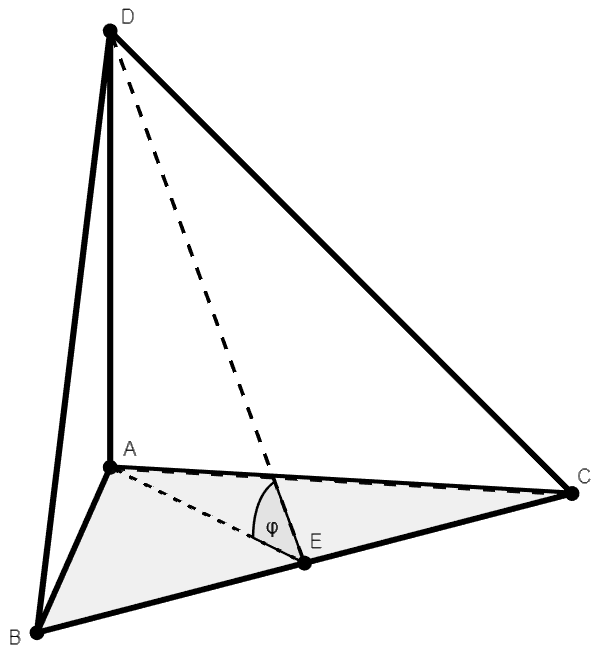
\includegraphics[scale=0.3]{Tetraeder1}
			\caption{Der Tetraeder $T_1$}
			\label{Abb.5}
		\end{minipage}
		\begin{minipage}[m]{0.4\textwidth}
			\hspace{1cm}
			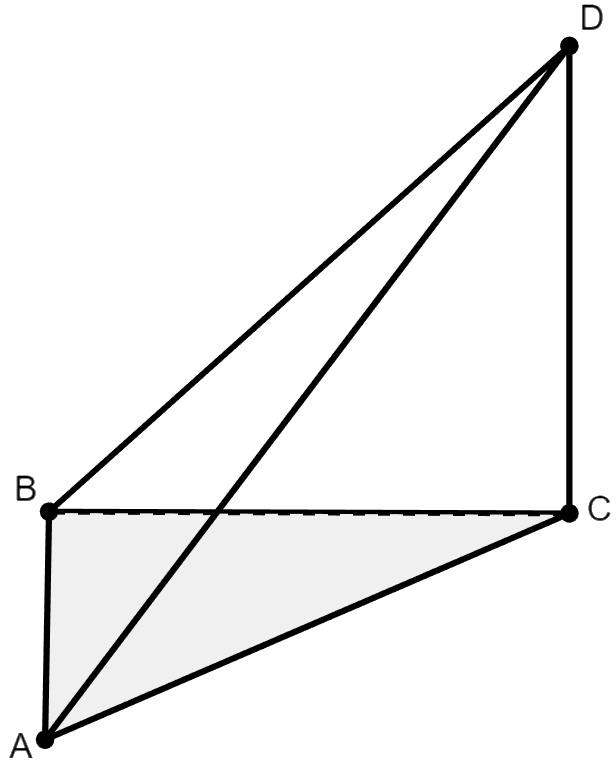
\includegraphics[scale=0.311]{Tetraeder2.1}
			\caption{Der Tetraeder $T_2$}
			\label{Abb.6}
		\end{minipage}
	\end{figure}

	\begin{example}
		Sei $T_2$ ein Tetraeder mit drei aufeinander folgenden Kanten 
		$\overline{AB}$, $\overline{BC}$ und $\overline{CD}$, die jeweils 
		orthogonal aufeinander stehen und die gleiche Länge $l$ haben. 
		Siehe dazu Abbildung \ref{Abb.6}. 
		Der Tetraeder $T_2$ hat die Grundseite $ABC$ und die Höhe $l$. 
		Drei der Diederwinkel haben hierbei den Wert $\frac{\pi}{2}$, 
		zwei den Wert $\frac{\pi}{4}$ und einer den Wert $\frac{\pi}{3}$. 
		Damit liegen alle Diederwinkel von $T_2$ in $\pi\setQ$ und damit 
		gilt 
		\[D(T_2)=0.\]
	\end{example}
	
	Wir sehen, dass die beiden Tetraeder $T_1$ und $T_2$ die 
	gleiche Grundseite und Höhe haben, jedoch unterschiedliche Dehn-Invarianten. 
	Damit sind sie nicht zerlegungsgleich. Wir haben also die vollständige 
	Lösung für Hilberts drittes Problem für die Zerlegungsgleichheit von 
	Polyeder gefunden.
	
	\newpage
	
	\section{Ergänzungsgleichheit von Polytopen}
	
	Wir wollen uns nun dem zweiten Teil von Hilberts Problem widmen und zwar der 
	Ergänzungsgleichheit von Polytopen. In diesem Kapitel zeigen wir, dass 
	Zerlegungsgleichheit und Ergänzungsgleichheit gleichbedeutend sind. Für den 
	Beweis hierzu benötigen wir vorweg noch einige Kenntnisse über Polytope. Das Kapitel richtet sich nach 
	\cite{Hadwiger}. 
	
	\subsection{Ein wenig Polyedertheorie}
	
	Wir beginnen mit dem einfachsten Polytop, dem Simplex. Ein Simplex 
	im $\setR^d$ hat 
	$d+1$ Ecken und damit gerade soviele Kanten, dass 
	wir ein konvexes Polytop erhalten. Im zwei-dimensionalen Fall ist ein 
	Simplex ein Dreieck und im drei-dimensionalen ein Tetraeder. Wir werden 
	feststellen, dass sich jedes konvexe Polytop in endlich viele Simplizes 
	zerlegen lässt. Diese Simplizialzerlegung von Polytopen spielt bei 
	der Zerlegungsgleichheit von Polytopen eine wichtige Rolle, wie wir schon im 
	Beweis des Bolyai-Gerwien Theorems (Satz \ref{theorem:bolyai-gerwien}) 
	gesehen haben. Ebenso ist, wie sich aus Hilberts Formulierung des 
	dritten Problems herauslesen lässt, ersichtlich, dass es eine der einfachsten Lösungen ist, zwei Simplizes mit gleichem Volumen zu finden, die nicht zerlegungsgleich sind.
	
	\begin{definition}[Simplex]\label{def:simplex}
		Ein \textsl{Simplex} $S$ im $\setR^d$ ist die konvexe Hülle einer Menge von 
		$d+1$ Punkten 
		$p_0,\ldots,p_d$, die sich im Raum in allgemeiner Lage befinden, also 
		nicht alle in einer Ebene liegen. Diese Punkte bezeichnen wir als 
		\textsl{Ecken} des Simplex. Wir wollen das Simplex durch Wahl der 
		Ecke $p=p_0$ und der Kantenvektoren 
		$s_i=p_i -p_{i-1}$ für alle $i=1,\ldots,d$ charakterisieren. 
		Wir schreiben für das Simplex S auch
		\[S=\langle p;s_1\ldots s_d\rangle.\]
	\end{definition}
	
	Ein Simplex ist offensichtlich ein spezielles konvexes Polytop. 
	
	\begin{remark}[Parameterdarstellung des Simplex]\label{bem:paradarst;simplex}
		Für einen Simplex $S=\langle p;s_1,\ldots s_d\rangle$ stellen wir 
		fest, dass sich jeder Punkt $s$ des Simplex in folgender Form darstellen 
		lässt
		\[s=p+\sum_{i=1}^d \alpha_i s_i\]
		für Parameter $1\geq \alpha_1\geq\ldots\geq\alpha_d\geq 0$. 
	\end{remark}
	
	\begin{theorem}[Simplizialzerlegung von Polytopen]\label{thm:simplzerl}
		Sei $P$ ein Polytop, dann lässt sich $P$ in endlich viele 
		Simplizes $S_1,\ldots,S_n$ zerlegen, das heißt
		\[P=S_1+\ldots+S_n.\]
	\end{theorem}
	
	\begin{proof}
		Das Polytop $P$ lässt sich nach Definition als Vereinigung endlich 
		vieler konvexer Polytope darstellen. Wir müssen also 
		zeigen, dass sich jedes konvexe Polytop $P'$ in endlich viele Simplizes 
		zerlegen lässt. Wir wollen dies per Induktion über die Dimension 
		des umgebenen Vektorraumes zeigen. Für $d=1$ ist die Aussage klar, da 
		jedes konvexe $1$-Polytop eine Strecke ist und damit auch ein 
		Simplex. Wir nehmen also an, die Aussage sei für die Dimension $d-1$ 
		bewiesen. Betrachten wir eine beliebige $d-1$-dimensionale Seite von 
		$P'$, dann wissen wir nach Induktionsvoraussetzung, dass sich diese  
		in endliche viele $d-1$-dimensionale Simplizes $S_1',\ldots,S_m'$ 
		zerlegen lassen. 
		Betrachten wir einen beliebigen festen Punkt $p'$ im Inneren von $P'$, dann 
		bildet für alle $i=1,\ldots,m$ die konvexe Hülle des Punktes $p'$ und 
		des Simplex $S_i'$ ein 
		neues $d$-dimensionales Simplex $S_i$. Führen wir das mit $p'$ auf 
		alle Seiten 
		von $P'$ fort, so erhalten wir eine, wegen der Konvexität 
		von $P'$, disjunkte 
		Zerlegung von $P'$ in endlich viele 
		Simplizes. Weiter erhalten wir demzufolge auch eine Zerlegung von 
		$P$ in Simplizes.
	\end{proof}
	
	Wir wollen uns zunächst überlegen, wie wir Polytope vervielfältigen, sowie 
	über eine Dilatation stauchen und strecken können. 
	
	\begin{definition}[Dilatation]
		Unter einer \textsl{Dilatation} mit einem Faktor $\lambda>0$ 
		verstehen wir eine Streckung bzw. Stauchung aller Punkte 
		im Koordinatensystem. Ein Punkt $p\in\setR^d$ wird auf 
		sein skalares Vielfaches $\lambda\cdot p$ abgebildet. In Bezug auf 
		Polytope erhalten wir mit dem Faktor $\lambda$ das dilatierte Polytop 
		\[\lambda P=\{\lambda p\ \vert\ p\in P\}.\]
	\end{definition}
	
	Wir bemerken, dass diese Abbildung, angewandt auf Polytope, wieder neue 
	Polytope erzeugt, da Halbräume auf Halbräume abgebildet werden. 
	Eine Dilatation um den Faktor $\lambda=1$ lässt die Punkte unverändert und 
	hat somit keine Auswirkung. 
	
	\begin{remark}\label{bem:dilvol}
		Gegeben $\lambda >0$. Dann können wir eine Dilatation mittels der Matrix
		\[M=\begin{pmatrix}
		\lambda &\ & 0\\
		\ &\ddots &\ \\
		0 &\ &\lambda
		\end{pmatrix}\] 
		bezüglich der Standardbasis des $\setR^d$ darstellen. Für das Volumen 
		eines Polytops $P$ erhält man mit 
		der Transformationsformel aus der Analysis (siehe auch \cite[Satz 4.7]{SkriptAna3})
		\[vol(\lambda P)=\abs{det(M)}\cdot vol(P)=\lambda^d\cdot vol(P).\]
	\end{remark}
	
	Weiter stellen wir fest, dass eine Streckung einer Zerlegung eines 
	Polytops das Gleiche ist wie die Zerlegung der gestreckten Polytope.
	
	\begin{lemma} \label{lemma:dilzerl}
		Sei $P$ ein Polytop und $P_1,\ldots,P_n$ endlich viele Polytope, s.~d. 
		$P=P_1+\ldots+P_n$ und $\lambda>0$ gegeben, dann gilt 
		\[\lambda P=\lambda P_1+\ldots+\lambda P_n.\]
	\end{lemma}
	
	\begin{proof}
		Es gilt
		\begin{align*}
			\lambda P&=\lambda(P_1+\ldots+P_n)\\
			&=\{\lambda p\ \vert\ p\in P_1 	\lor\ldots\lor p\in P_n\}\\
			&=\{\lambda p\ \vert\ p\in P_1\}\cup\ldots\cup
			\{\lambda p\ \vert\ p\in P_n\}\\
			&=\lambda P_1 +\ldots+\lambda P_n.
		\end{align*}
	\end{proof}
	
	\begin{lemma} \label{lemma:dilkong}
		Seien $P$ und $Q$ zwei Polytope und $\lambda>0$ gegeben, dann gilt 
		$P\cong Q$ genau dann, wenn $\lambda P\cong \lambda Q$.
	\end{lemma}
	
	\begin{proof}
		Seien für die Hinrichtung $P\cong Q$ gegeben. Somit gibt es eine Isometrie 
		$f$, s.~d. gilt $f(P)=Q$. Wir können die Isometrie $f$ durch ein $\alpha\in
		\setR^d$ und eine orthogonale Matrix $U\in O(d)$ darstellen, s.~d. 
		$f(P)=\alpha + UP$ gilt. Betrachte die Isometrie $f_{\lambda}$, die 
		für alle $x\in\setR^d$ durch 
		$f_{\lambda}(x)=\lambda\cdot \alpha +Ux$ definieren. 
		Offensichtlich ist $f_{\lambda}$ wieder eine Isometrie. 
		Dann gilt
		\[f_{\lambda}(\lambda P)=\lambda\cdot \alpha+U \lambda P =\lambda\cdot 
		\alpha+\lambda U P =\lambda(\alpha+ U P)=\lambda f(P)=\lambda Q\]
		Damit sind $\lambda P$ und $\lambda Q$ kongruent. \\
		Seien für die Rückrichtung nun $\lambda P\cong \lambda Q$, folglich  
		gibt es eine Isometrie $f$, s.~d. $f(\lambda P)=\lambda Q$. Es gibt 
		also wieder $\alpha\in\setR^d$ und $U\in O(d)$, s.~d. 
		$f(x)=\alpha + Ux$ für alle $x\in\setR^d$ gilt. Betrachte die Isometrie 
		$f_{\lambda}$, die wir durch 
		$f_{\lambda}(x)=\frac{1}{\lambda}\cdot \alpha +U x$ für alle $x\in\setR^d$ 
		definieren. Diese ist wieder eine Isometrie. Dann gilt 
		\[f_{\lambda}(P)=\frac{1}{\lambda}\cdot \alpha +U P 
		=\frac{1}{\lambda}(\alpha+\lambda U P)
		=\frac{1}{\lambda}(\alpha + U \lambda P)
		=\frac{1}{\lambda} f(\lambda P)=\frac{1}{\lambda} \lambda Q =1\cdot Q=Q.\]
		Die Polytope $P$ und $Q$ sind demzufolge kongruent.
	\end{proof}
	
	\begin{proposition} \label{prop:dilzerl}
		Seien $P$ und $Q$ Polytope und $\lambda>0$ gegeben, dann gilt 
		$P\sim Q$ genau dann, wenn $\lambda P\sim \lambda Q$.
	\end{proposition}
	
	\begin{proof}
		Seien für die Hinrichtung $P$ und $Q$ zerlegungsgleich, dann gibt 
		es endlich viele Polytope $P_1,\ldots,P_n$ und $Q_1\ldots,Q_n$ mit 
		$P=P_1+\ldots+P_n$ und $Q=Q_1+\ldots Q_n$, s.~d. $P_i\cong Q_i$ 
		für alle $i=1,\ldots, n$. Nach Lemma \ref{lemma:dilzerl} können wir 
		die Zerlegungen der gestreckten Polytope betrachten, also
		\begin{align*}
			\lambda P&=\lambda (P_1+\ldots P_n)=\lambda P_1 +\ldots+\lambda P_n \\
			\lambda Q&=\lambda (Q_1+\ldots Q_n)=\lambda Q_1 +\ldots+\lambda Q_n.
		\end{align*}
		Weiter gilt mit Lemma \ref{lemma:dilkong}, dass aus $P_i\cong Q_i$ 
		für alle $i=1,\ldots,n$ folgt, dass auch $\lambda P_i\cong\lambda Q_i$ 
		für alle $i=1,\ldots,n$ gilt. Damit folgt $\lambda P\sim \lambda Q$. \\
		Für die Rückrichtung seien $\lambda P\sim \lambda Q$, dann gibt 
		endlich viele Polytop $P_1,\ldots P_n$ und $Q_1\ldots Q_n$ mit 
		$\lambda P=P_1+\ldots+P_n$ und $\lambda Q=Q_1+\ldots+Q_n$, s.~d. 
		$P_i\cong Q_i$ für alle $i=1,\ldots,n$. Wir betrachten die 
		Zerlegungen
		\begin{align*}
			P&=1\cdot P=\frac{1}{\lambda}\lambda P=\frac{1}{\lambda}(P_1+\ldots+P_n)
			=\frac{1}{\lambda}P_1+\ldots+\frac{1}{\lambda}P_n \\
			Q&=1\cdot Q=\frac{1}{\lambda}\lambda Q=\frac{1}{\lambda}(Q_1+\ldots+Q_n)
			=\frac{1}{\lambda}Q_1+\ldots+\frac{1}{\lambda}Q_n.
		\end{align*}
		Dann sind mit Lemma \ref{lemma:dilkong}, wegen der Kongruenz der $P_i$ und 
		$Q_i$ für alle $i=1,\ldots,n$, die Polytope $\frac{1}{\lambda}P_i$ und 
		$\frac{1}{\lambda}Q_i$ für alle $i=1,\ldots,n$ kongurent. 
		Die Polytope $P$ und $Q$ sind demnach zerlegungsgleich.
	\end{proof}
	
	\begin{definition}[Vervielfachung]
		Sei $P$ ein Polytop, dann ist die \textsl{ganze Vervielfachung} 
		von $P$ mit 
		einer natürlichen Zahl $n$ ein Polytop, wir schreiben $n\cdot P$, 
		das sich in $n$ viele Polytope zerlegen lässt, die alle kongruent zu 
		$P$ sind. Formal bedeutet das, dass es Polytope $P_1,\ldots,P_n$ gibt, s.~d.
		\[n\cdot P=P_1+\ldots+P_n,\]
		wobei $P_i\cong P$ für alle $i=1,\ldots,n$.
	\end{definition}
	
	Wir bemerken, dass die Lage und Ausrichtung der Polyeder $P_i$ nicht 
	eindeutig festgelegt 
	ist, was jedoch beim eigentlichen Zerlegen keine Rolle spielt. Wir wollen 
	die Polytope so verschieben, dass sie paarweise disjunkt sind.
	
	Es ergeben sich beim Vervielfältigen folgende Eigenschaften.
	
	\begin{remark}\label{bem:vervielf;vol}
		Wir wollen uns überlegen, wie sich das Volumen bei einer Vervielfachung 
		verhält. Dazu sei $P$ ein Polytop und $n$ eine natürliche Zahl. 
		Das Polytop $n\cdot P$ lässt sich in endlich viele Polytope 
		$P_1,\ldots,P_n$ zerlegen, also $n\cdot P=P_1+\ldots+P_n$ und für alle 
		$i=1,\ldots,n$ soll $P_i\cong P$ gelten. Mit Proposition 
		\ref{prop:cong,vol} gilt dann 
		\[vol(n\cdot P)=vol(P_1+\ldots+P_n)=vol(P_1)+\ldots+vol(P_n)=n\cdot vol(P).\]
	\end{remark}
	
	\begin{remark}[Additionssatz] \label{bem:addsatz}
		Seien $P,Q,R,S$ vier Polytope, s.~d. $P\sim Q$ und $R\sim S$, dann gilt
		\[P+R\sim Q+S.\]
		Wir iterieren hierbei einfach die Zerlegungen der einzelnen Polytope 
		auf und erhalten damit die Zerlegungsgleichheit.
	\end{remark}
	
	\begin{remark}[Multiplikationssatz] \label{bem:multsatz}
		Seien $P$ und $Q$ zwei Polytope und $n$ eine natürliche Zahl. 
		Dann sind die Polytope $n\cdot P$ und $n\cdot Q$ zerlegungsgleich, falls 
		$P$ und $Q$ zerlegungsgleich sind.
	\end{remark}
	
	\begin{corollary} \label{coroll:vervielfältigung}
		Seien $P$ und $Q$ zwei Polytope und $n$ eine natürliche Zahl, dann gilt
		\[n\cdot(P+Q)\sim n\cdot P+n\cdot Q.\]
	\end{corollary}
	
	\begin{proof}
		Wir finden $n$ viele Polytope $R_1,\ldots,R_n$ mit 
		$R_i\cong (P+Q)$ für alle $i=1,\ldots,n$, s.~d. 
		$n\cdot(P+Q)=R_1+\ldots+R_n$. Da Schnitte von Polytopen wieder 
		Polytope sind, folgt, dass sich jedes 
		$R_i$ darstellen lässt durch Polytope $P_i$ und $Q_i$ für alle 
		$i=1,\ldots,n$, wobei $P_i\cong P$ und $Q_i\cong Q$. Ebenso finden wir 
		mit der Definition der Polytope $n\cdot P$ und $n\cdot Q$ auch jeweils 
		$n$ viele Polytope 
		$P_1',\ldots,P_n'$ und $Q_1',\ldots,Q_n'$ mit $P_i'\cong P$ und 
		$Q_i'\cong Q$ für alle $i=1,\ldots,n$, s.~d. $n\cdot P=P_1'+\ldots+P_n'$ und 
		$n\cdot Q=Q_1'+\ldots+Q_n'$. Mit der Transitivität der Kongruenz 
		gilt auch $P_i\cong P_i'$ und $Q_i\cong Q_i'$ für alle 
		$i=1,\ldots,n$. Wir erhalten die Zerlegungen
		\begin{align*}
		n\cdot(P+Q)&=R_1+\ldots+R_n=P_1+Q_1+\ldots+P_n+Q_n \qquad\text{und}\\
		n\cdot P+n\cdot Q&=P_1'+\ldots+P_n'+Q_1'+\ldots+Q_n'=
		P_1'+Q_1'+\ldots+P_n'+Q_n'.
		\end{align*}
		Damit sind $n\cdot (P+Q)$ und $n\cdot P+n\cdot Q$ zerlegungsgleich.
	\end{proof}

	Um Polytope besser zu charakterisieren, werden wir in diesem Abschnitt 
	sogenannte Zylinderklassen einführen. Wir werden später feststellen, 
	dass diese Charakterisierung beim Beweisen einiger Resultate sehr 
	hilfreich ist.

	\subsection{Zylinderklassen}
	
	\begin{definition}[Minkowski-Summe]
		Seien $A$ und $B$ Mengen, dann ist die \textsl{Minkowski-Summe} $A\times B$ 
		von $A$ und $B$ mit der vektoriellen Addition definiert als
		\[A\times B=\left.\{a+b\ \right\vert\ a\in A,b\in B\}.\]
		In Bezug auf die leere Menge gilt
		\[A\times \emptyset =\emptyset\times A=\emptyset.\]
	\end{definition}
	
	\begin{remark} \label{bem:mink}
		Seien $A,B,C$ Mengen, dann ergeben sich folgende Eigenschaften 
		mit der Minkowski-Summe.
		\begin{enumerate}
			\item Die Minkowski-Addition erbt die Kommutativität und Assoziativität von der Addtion, d.~h. 
			es gilt
			\[A\times B=B\times A\qquad\text{und}\qquad A\times(B\times C)=(A\times B)\times C.\]
			
			\item \label{bem:mink;3} 
			Weiter gelten auch die Distributivgesetze, also 
			\[(A\cup B)\times C=(A\times C)\cup (B\times C)\]
			und mit der Kommutativität der Minkowski-Addition erhalten wir das zweite 
			Distributivgesetz. Wenden wir dies nun auf Polytope 
			$P,Q$ und $R$ an, dann gilt
			\begin{align}
			(P+Q)\times R =(P\times R)+(Q\times R)\quad\text{und}\quad
			P\times (Q+R)=(P\times Q)+(P\times R).
			\end{align}
			\item \label{bem:mink;1}In Verbindung mit der Dilatation ergibt sich für Polytope 
			$P$ und $Q$ und ein $\lambda>0$, dass
			\[\lambda P\times \lambda Q=\lambda(P\times Q)\]
			gilt.
			\item \label{bem:mink;2} 
			Wir hatten im Zusammenhang mit der Definition der 
			Kongruenz \ref{def:kong} bereits die Translationsgruppe 
			erwähnt, die Untergruppe der Isometriegruppe, welche ausschließlich 
			aus Translationen besteht. Wir stellen fest, dass für zwei 
			Translationen $f,g$ im Zusammenhang mit der Minkowski-Summe 
			\[f(A)\times g(B)=(g\circ f)(A\times B)\]
			gilt (siehe dazu auch \cite{Hadwiger}[1.2.2]).
		\end{enumerate}
	\end{remark}
	
	\begin{definition}[Parallelotop]
		Seien $p_1,\ldots,p_d$ linear unabhängige Vektoren und $S_1,\ldots,S_d$ 
		die durch die Vektoren $p_1,\ldots,p_d$ für alle $i=1,\ldots,n$ 
		definierten Strecken
		\[S_i=\{tp_i\ \vert\ t\in[0,1]\},\]
		die die Richtung und Länge der Vektoren $p_1,\ldots,p_d$ 
		haben. Dann ist das \textsl{Parallelotop} $P$ definiert durch 
		\[P=S_1\times\ldots\times S_d.\]
		Wir sagen, das Parallelotop wird durch die Vektoren $p_1,\ldots,p_d$ 
		erzeugt.
	\end{definition}
	
	\begin{definition}[Gramsches Funktional]
		Sei $P$ das durch die Vektoren $p_1,\ldots,p_d$ 
		erzeugte Parallelotop, dann ordnen wir dem Parallelotop $P$ das 
		\textsl{Gramsche Funktional} $\mathfrak{D}(P)>0$ zu, das definiert ist durch
		\[\mathfrak{D}(P)=\left(det \begin{pmatrix}
		\langle p_1,p_1\rangle & \cdots &\langle p_1,p_d\rangle \\
		\vdots & \ddots & \vdots \\
		\langle p_d,p_1 \rangle & \cdots & \langle p_d,p_d \rangle
		\end{pmatrix}\right)^{1/2}.\]
	\end{definition}
	
	Wir meinen mit $\langle p_i,p_j\rangle$ hier das Standardskalarprodukt. 
	
	\begin{remark} \label{bem:gramfunk}
		Wir stellen fest, dass das Gramsche Funktional folgende Eigenschaften 
		erfüllt.
		\begin{enumerate}
			\item Sind $P$ und $Q$ zwei kongruente Parallelotope, dann gilt mit 
			der Invarianz des Skalarprodukts unter Isometrien
			\[\mathfrak{D}(P)=\mathfrak{D}(Q).\]
			\item \label{bem:gramfunk;2} Sei $P$ ein Parallelotop und $\lambda>0$ gegeben, dann gilt 
			\[\mathfrak{D}(\lambda P)=\lambda^d \mathfrak{D}(P).\]
		\end{enumerate}
	\end{remark}
	
	\begin{theorem} \label{thm:zerlgram}
		Die Parallelotope $P$ und $Q$ sind zerlegungsgleich, falls ihre 
		Gramschen Funktionale übereinstimmen, d.~h. $\mathfrak{D}(P)=\mathfrak{D}(Q)$.
	\end{theorem}
	
	\begin{proof}
		Beweisskizze: Der Beweis des Satzes ergibt sich aus zwei 
		Resultaten. Es lässt sich feststellen, dass zwei Parallelotope 
		scherungsäquivalent sind, falls ihre Gramschen Funktionale übereinstimmen. 
		Vergleiche mit \cite{Hadwiger}[Kapitel 1, Satz III].
		Mit scherungsäquivalent meinen wir hier, dass wir die 
		Vektoren, die die Parallelotope erzeugen, so verändern, dass wir 
		in endlich vielen Scherungen die Parallelotope ineinander 
		überführen können. Bei einer Scherung addieren wir auf einen 
		dieser Vektoren ein Vielfaches eines anderen Vektors von diesen.
		Weiter kann man aus der Scherungsäquivalenz der Parallelotope folgern, 
		dass diese auch zerlegungsgleich sind. Siehe dazu 
		\cite{Hadwiger}[Kapitel 1,Satz IV].
	\end{proof}
	
	\begin{definition}[$i$-stufiger Zylinder]
		Ein Polytop $P$ ist ein $i$-\textsl{stufiger Zylinder}, falls es eine Darstellung 
		der Form
		\[P=P_1 \times\ldots\times P_i\]
		gibt, wobei $P_k$ für alle $k=1,\ldots,i$ konvexe Polytope sind, die jeweils in einer $d_k$-dimensionalen Ebene $E_{d_k}$ liegen. Hierbei soll $\sum_{k=1}^i d_k =d$ und $d_k\geq 1$ für alle $k=1,\ldots,i$ 
		gelten. Die Ebenen $E_{d_k}$ befinden sich paarweise in allgemeiner Lage, d.~h. dass diese paarweise keine gleichen Richtungen aufweisen 
		bzw. als Räume komplementär in $\setR^d$ liegen.
	\end{definition}
	
	Wir bemerken, dass die konvexen Polytope $P_1,\ldots,P_n$ uneigentliche 
	Polytope sind. Dennoch gibt es die Möglichkeit, diese in ihrer Ebene 
	$E_{d_k}$ als ein eigentliches Polytop aufzufassen.
	
	Jedes Simplex ist also offensichtlich ein $1$-stufiger Zylinder. Genauso 
	ist jedes Parallelotop ein $k$-stufiger Zylinder. 
	
	\begin{definition}[Zylinderklassen]
		Ein Polytop $P$ ist ein $i$-\textsl{stufiges Zylinderpolytop}, falls 
		es endlich viele $i$-stufige Zylinder $P_1,\ldots,P_n$ gibt, s.~d.
		\[P=P_1+\ldots+P_n.\]
		Die $i$-\textsl{te Zylinderklasse} $\mathfrak{B}_i$ ist die Menge aller 
		Polytope, die zu einem $i$-stufigen Zylinderpolytop zerlegungsgleich 
		sind, wobei $\emptyset\in\mathfrak{B}_i$. 
		Die Stufenzahl $i$, mit $1\leq i\leq  d$, ist die Ordnung 
		der Zylinderklasse $\mathfrak{B}_i$.
	\end{definition}
	
	Es ist klar, dass für zwei Polytope $P,Q\in \mathfrak{B}_i$ 
	auch $P+Q\in\mathfrak{B}_i$ gilt. 
	Besonders interessant sind hierbei die erste und die $d$-te Zylinderklasse. 
	Es lässt sich nämlich feststellen, dass die erste Zylinderklasse gerade 
	der Menge aller Polytope entspricht. Jedes Polytop lässt sich nach Satz  
	\ref{thm:simplzerl} in endlich viele Simplizes zerlegen und jedes Simplex ist ein $1$-stufiger Zylinder. 
	Die $d$-te Zylinderklasse entspricht gerade Polytopen, welche mit endlich vielen 
	Parallelotopen zerlegungsgleich sind. Es gilt sogar die folgende Eigenschaft.
	
	\begin{proposition} \label{bem:dteZylinderklasse}
		Sei $P\in\mathfrak{B}_d$ ein Polytop, dann gibt es ein $\lambda>0$, s.~d. 
		\[P\sim \lambda W.\] 
	\end{proposition}
	
	Hierbei ist $W$ der $d$-dimensionale Einheitswürfel, den wir erhalten, 
	indem wir die Minkowski-Summe der Strecken $S_1,\ldots,S_n$, 
	welche die Richtung und Länge der Standardbasisvektoren $e_1,\ldots, e_d$ 
	des $\setR^d$ haben, bilden.
	
	\begin{proof}
		Da $P$ ein Polytop aus der $d$-ten Zylinderklasse ist, finden 
		wir endlich viele Parallelotope $P_1,\ldots, P_n$, s.~d. 
		$P=P_1+\ldots+P_n$. Wir definieren $\lambda$ durch 
		\[\lambda^d =\sum_{i=1}^n \mathfrak{D}(P_i).\]
		Weiter definieren wir 
		\begin{align}
			\lambda_i =\frac{\mathfrak{D}(P_i)}{\lambda^d} \label{thm:dtezyl;1}
		\end{align}
		für alle $i=1,\ldots,n$. Dann lässt sich der Einheitswürfel $W$ in $n$ viele 
		Parallelotope $W_1,\ldots,W_n$ zerlegen, wobei
		\[W_i:=(S_1\times\ldots S_{d-1}\times \lambda_i S_d)+
		\sum_{k=1}^{i-1} \lambda_k e_d\]
		für alle $i=1,\ldots,n$ gilt. Anschaulich wird der Einheitswürfel $W$  hierbei in $n$ viele Scheiben der Länge $\lambda_i$ geschnitten. 
		Es gilt 
		\[\mathfrak{D}(\lambda W_i)=\lambda^d \mathfrak{D}(W_i)=
		\lambda^d \left(det \left(\begin{smallmatrix}
		1 & \ &\ &0 \\
		\ &\ddots &\ &\ \\
		\ & \ &  1 &\ \\
		0 & \ & \ & \lambda_i
		\end{smallmatrix}\right)\right)^{1/2}=\lambda^d \lambda_i\overset{\ref{thm:dtezyl;1}}{=}\mathfrak{D}(P_i)\]
		für alle $i=1,\ldots,n$. Mit Satz \ref{thm:zerlgram} 
		sind also $P_i$ und $\lambda W_i$ für alle $i=1,\ldots,n$ zerlegungsgleich. 
		Mit dem Additionssatz (Satz \ref{bem:addsatz}) 
		sind auch $P$ und $\lambda W$ zerlegungsgleich.
	\end{proof}
	
	\begin{remark}
		Wir stellen fest, dass jeder $i$-stufige Zylinder auch ein $j$-stufiger 
		Zylinder für ein $j<i$ ist und damit erhalten wir
		\[\mathfrak{B}_1\supset \mathfrak{B}_2\supset \ldots\supset\mathfrak{B}_d.\]
	\end{remark}
	
	Die Zylinderklassen sind vor allem deswegen für uns interessant, da sie 
	Beweisverfahren nach dem Prinzip der vollständigen Induktion ermöglichen. 
	So können wir Aussagen für alle Polytope mittels Induktion über die 
	Zylinderklassen beweisen. Wir werden dieses Verfahren im Beweis zu Satz 
	\ref{thm:zerlerg} verwenden. Im nächsten Abschnitt werden wir uns 
	einen Hilfssatz anschauen, der die Dilatation von Polytopen 
	in Verbindung mit der Vervielfachung von Polytopen bringen wird. 
	Wir werden sehen, dass dieser Satz von zentraler Bedeutung für 
	die darauffolgenden Beweise ist.
	
	\subsection{Hilfssatz}
	
	Wir wollen noch die Translationsgleichheit, analog zur Kongruenz, 
	von Polytopen einführen. 
	Dazu erinnern wir uns an die Translationsgruppe.  
	Wir benötigen an einigen Stellen in den Beweisen in diesem Abschnitt 
	die Translationsgleichheit. Letztendlich können wir dann den Hilfssatz 
	auf die Zerlegungsgleichheit verallgemeinern, da die translative 
	Zerlegungsgleichheit die Zerlegungsgleichheit impliziert.
	
	\begin{definition}[Translationsgleichheit, translative Zerlegungsgleichheit]
		Wir nennen zwei Polytope $P$ und $Q$ \textsl{translationsgleich}, wenn es 
		eine Translation $f$ aus der Translationsgruppe gibt, s.~d. 
		$f(P)=Q$ gilt. Wir schreiben $P\cong_t Q$. \\
		Die Translationsgleichheit ist wie die Kongruenz eine 
		Äquivalenzrelation. \\
		Weiter nennen wir zwei Polytope $P$ und $Q$ \textsl{translativ 
		zerlegungsgleich}, wenn es endlich viele $P_1,\ldots,P_n$ und 
		$Q_1,\ldots,Q_n$ gibt, mit $P=P_1+\ldots+P_n$ und $Q=Q_1+\ldots+Q_n$, s.~d. 
		für alle $i=1,\ldots,n$ die Polytope $P_i$ und $Q_i$ translationsgleich 
		sind. Wir schreiben $P\approx Q$.
	\end{definition}
	
	\begin{remark}
		Es ist klar, dass aus der Translationsgleichheit von Polytopen auch die 
		Kongruenz folgt. Damit folgt aus der translativen Zerlegungsgleichheit 
		die Zerlegungsgleichheit. Wir bemerken, dass die Eigenschaften 
		in diesem Kapitel, 
		die wir für die Zerlegungsgleichheit gezeigt haben, 
		auch für die translative Zerlegungsgleichheit gelten. 
	\end{remark}
	
	Weiter erhalten wir mit Bemerkung \ref{bem:mink} Eigenschaft \ref{bem:mink;2} 
	auch die folgende Eigenschaft.
	\begin{remark}\label{bem:mink;zerl}
		Seien $P,Q,R,S$ Polytope mit $P\approx R$ und $Q\approx S$, dann gilt 
		$P\times Q\approx R\times S$. \\
		Betrachten wir die Zerlegungen der einzelnen Polytope und setzen diese in 
		$P\times Q$ und $R\times S$ ein. Dann ergeben sich durch Ausmultiplizieren 
		mit den Distrubivgesetzen der Minkowski-Addition Zerlegungen, dessen 
		einzelne Polytope mit Bemerkung 
		\ref{bem:mink} Eigenschaft \ref{bem:mink;2} translationsgleich sind.
	\end{remark}
	
	Bevor wir zu dem Hilfssatz kommen, wollen wir uns eine Folgerung aus der kanonischen 
	Simplexzerlegung anschauen. 
		
	\begin{definition}[Simplotop]
		Sei $p$ ein Vektor und  $s_1\ldots,s_i$ und 
		$t_1,\ldots,t_{d-i}$ insgesamt 
		$d$ linear unabhängige Vektoren, wobei $1\leq i\leq d-1$ ist. Dann ist 
		das \textsl{Simplotop} $S$ gerade das Polytop, dessen Elemente $s$ 
		dargestellt werden durch
		\[s=p+\sum_{k=1}^i \alpha_k s_k +\sum_{j=1}^{d-i}\beta_j t_j,\]
		für beliebige $1\geq \alpha_1\geq\ldots\geq\alpha_i\geq 0$ und 
		$1\geq \beta_1\geq\ldots\geq\beta_{d-i}\geq 0$.
	\end{definition}
	
	Erinnern wir uns zurück an die Definition des Simplex (Definition \ref{def:simplex}) dann fallen uns in dieser Definition einige Gemeinsamkeiten 
	auf. Tatsächlich ergibt sich die folgende Bemerkung.
	
	\begin{remark}
		Wir stellen fest, dass wir ein wie oben definiertes Simplotop $S$ 
		als Minkowski-Summe eines Punktes $p$ und zweier 
		im Ursprung liegender Simplexe $S_1=\langle 0;s_1,\ldots,s_i\rangle$ 
		und $S_2=\langle 0;t_1\ldots,t_{d-i}\rangle$ darstellen lässt. 
		Es gilt also 
		\[S=p\times S_1 \times S_2.\]
	\end{remark}
	
	Wir betrachten nun die Zerlegung eines Simplex in $d+1$ viele konvexe 
	Teilpolytope, die sogenannte kanonische Simplexzerlegung. 
	
	\begin{theorem}[Folgerung aus der Kanonischen Simplexzerlegung]\label{thm:kanonsimpl}
		Sei $S$ ein Simplex und $0<\lambda<1$ gegeben, dann 
		gibt es ein $S_0\in\mathfrak{B}_2$, s.~d.
		\[S\approx \lambda S+(1-\lambda)S +S_0.\]
	\end{theorem}
	
	Dieser Satz ist ein spezielles Resultat aus der Kanonischen Simplexzerlegung 
	in \cite{Hadwiger}[1.2.6]. Wir wollen uns aus dem Beweis an dieser 
	Stelle nur die Konstruktion, mit 
	der wir auf die Zerlegungsrelation kommen, anschauen, den vollständigen 
	Beweis jedoch nicht.
	
	\begin{proof}
		Sei $S=\langle p;s_1\ldots,s_d\rangle$ das Simplex und 
		$0<\lambda<1$ gegeben. Wir wollen 
		zunächst diesem Simplex für alle $i=1,\ldots,d-1$ zwei 
		uneigentliche Simplexe $S_i'=\langle p;s_1,\ldots,s_i\rangle$ und 
		$S_{d-i}''=\langle p+\sum_{k=1}^i s_k ;s_{i+1},\ldots,s_d\rangle$ 
		zuordnen. Die beiden Simplexe $S_i'$ und $S_{d-i}''$ liegen 
		in allgemeiner Lage in komplementären Räumen. Wir ergänzen 
		unsere Konstruktion durch $S_0'=p$, $S_0''=q=p+\sum_{k=1}^i s_k$ und 
		$S_d'=S_d''=S$. Seien nun die Simplotope 
		$W_0(\lambda),\ldots,W_d(\lambda)$ gegeben durch
		\[W_i(\lambda)=(1-\lambda)S_i' \times \lambda S_{d-i}''\]
		für alle $i=0,\ldots,d$. Besonders das erste und letzte Simplotop 
		sind hierbei interessant. Es gilt nämlich 
		$W_0(\lambda)=(1-\lambda)p\times \lambda S$, was translationsgleich 
		zu $\lambda S$ ist, und $W_d(\lambda)=\lambda q\times (1-\lambda) S$, 
		was translationsgleich zu $(1-\lambda)S$ ist. Damit gilt dann 
		die Zerlegung
		\[S=W_0(\lambda)+\ldots+W_d(\lambda).\]
		Dieses Resultat ist die kanonische Simplexzerlegung. Für den Beweis 
		davon sei auf \cite{Hadwiger}[1.2.6] verwiesen. 
		Wir stellen fest, dass die Simplotope $W_1(\lambda),\ldots,W_{d-1}(\lambda)$, als 
		Minkowski-Summe zweier uneigentlicher Simplexe, alle $2$-stufige Zylinder 
		sind und damit in $\mathfrak{B}_2$ liegen. Damit auch 
		$W_1(\lambda)+\ldots+W_{d-1}(\lambda)\in\mathfrak{B}_2$. Wir 
		definieren also $S_0=W_1(\lambda)+\ldots+W_{d-1}(\lambda)$. 
		Weiter gilt $W_0(\lambda)\approx \lambda S$ und 
		$W_d(\lambda)\approx (1-\lambda)S$ demnach erhalten wir
		\[S=W_0(\lambda)+\ldots+W_d(\lambda)\approx \lambda S+(1-\lambda)S+S_0.\]
	\end{proof}
	
	\begin{theorem}[Hilfssatz]\label{thm:hilfssatz}
		Sei $P$ ein Polytop, das in der $i$-ten Zylinderklasse $\mathfrak{B}_i$ ist 
		und $n$ eine natürliche Zahl, dann gilt
		\[nP\sim n^i\cdot P+P_0,\]
		wobei $P_0\in\mathfrak{B}_{i+1}$ ein (von $n$ abhängiges) Polytop ist. 
		Falls $i=d$ ist $P_0=\emptyset$.
	\end{theorem}
	
	Da wir im Beweis der Aussage lediglich die Streckung und Vervielfachung 
	von Polytopen betrachten, gilt der Satz sogar für translative Zerlegungsgleichheit, 
	wir folgern daraus die Zerlegungsgleichheit.
	
	\begin{proof}
		\noindent
		\begin{enumerate}
			\item Fall: Es gilt $i=1$ dann reicht es, aufgrund 
			der Simplizialzerlegung eines Polytops, die 
			Behauptung für ein Simplex $P$ nachzuweisen. Für alle $j=1,\ldots,n-1$ 
			gilt nun, dass $n-j\in\{1,\ldots,n-1\}$ und $n-j+1\in\{2,\ldots,n\}$ 
			und damit auch $0<\frac{n-j}{n-j+1}<1$. Wir wenden nun  
			Satz \ref{thm:kanonsimpl} mit den Parametern 
			$\lambda_j=\frac{n-j}{n-j+1}$ an und 
			erhalten für alle $j=1,\ldots,n-1$ die Relationen 
			\[P\approx \frac{n-j}{n-j+1} P+\left(1-\frac{n-j}{n-j+1}\right)P+P_{j,0}
			=\frac{n-j}{n-j+1}P+\frac{1}{n-j+1}P+P_{j,0},\]
			wobei $P_{j,0}\in\mathfrak{B}_2$ gilt. Mit Dilatation mit 
			$n-j+1$ erhalten wir dann die Relationen 
			\begin{align*}
				(n-j +1)P\approx (n-j )P+P_j+P_{j, 0} 
			\end{align*}
			für alle $j=1,\ldots,n-1$, wobei $P_{j}\cong_t P$ und 
			$P_{j, 0}\in\mathfrak{B}_2$ gilt. Wir schreiben die Relationen 
			aus als
			\begin{align*}
				nP &\approx (n-1)P+P_1+P_{1,0} \\
				(n-1)P &\approx (n-2)P+P_2 +P_{2,0} \\
				&\ \vdots \\
				3P &\approx 2P +P_{n-2}+P_{n-2,0} \\
				2P &\approx P +P_{n-1}+P_{n-1,0}
			\end{align*}
			Es lässt sich durch sukzessives Einsetzen erkennen, dass wir 
			schreiben können 
			\[nP\approx (P+P_1+\ldots+P_{n-1})+(P_{1,0}+\ldots+P_{n-1,0}).\]
			Wir können die erste Summe zusammenfassen zu $n \cdot P$ 
			und da alle $P_{j,0}$ in $\mathfrak{B}_2$ liegen, liegt auch 
			die Summe in $\mathfrak{B}_2$ und wir erhalten
			\begin{align}
				nP\approx n\cdot P+ P_0 \label{thm:zyl;1}
			\end{align}
			für ein $P_0\in\mathfrak{B}_2$. Damit sind wir mit dem 
			ersten Fall fertig.
			
			\item Fall: Es gilt $i>1$, folglich reicht es die Behauptung für einen 
			$i$-stufigen Zylinder $P$ nachzuweisen. Sei also 
			$P=P_1\times\ldots \times P_i$ 
			für konvexe Polytope $P_1\ldots,P_i$ die in $d_k$-dimensionalen 
			Ebenen $E_{d_k}$ liegen, mit $\sum_{k=1}^i d_k =d$ und 
			$d_k\geq 1$ für alle $k=1,\ldots i$. 
			Es gilt mit Bemerkung \ref{bem:mink} Eigenschaft  
			\ref{bem:mink;1} auch 
			\[nP=nP_1\times\ldots\times nP_i.\]
			Betrachten wir Zylinderklassen in den Räumen $\setR^{d_k}$, in denen 
			die Ebenen $E_{d_k}$ liegen. Dann sind die konvexen Polytope 
			$P_1,\ldots,P_i$, die im Raum $\setR^d$ uneigentliche Polytope sind, 
			im Raum $\setR^{d_k}$ wieder eigentliche Polytope, die 
			wir als Polytope der Zylinderklasse $\mathfrak{B}_1^{(d_k)}$ 
			auffassen können. Mit $\mathfrak{B}_i^{(d_k)}$ meinen wir  
			die $i$-te Zylinderklasse der $d_k$-dimensionalen Polytope, die in 
			der Ebene $E_{d_k}$ liegen. Mit dem ersten Fall (Relation 
			\ref{thm:zyl;1}) folgt also für 
			die Polytope, dass für alle $k=1,\ldots,i$ gilt
			\[nP_k\approx P_{k,0}+n\cdot P_k=P_{k,0}+P_{k,1}+\ldots+P_{k,n},\]
			wobei $P_{k,0}\in \mathfrak{B}_2^{(d_k)}$ und $P_{k,j}\cong_t P_k$ 
			für alle $j =1,\ldots,n$ ist. Wir erhalten mit 
			Bemerkung \ref{bem:mink;zerl} die Relation 
			\[nP=nP_1\times\ldots\times nP_i \approx (P_{1,0}+P_{1,1}+\ldots+P_{1,n})
			\times\ldots\times (P_{i,0}+P_{i,1}+\ldots+P_{i,n}),\]
			die wir mit den Distributivgesetzen aus Bemerkung 
			\ref{bem:mink} \ref{bem:mink;3} 
			umformen können zu
			\[nP\approx \sum_{\genfrac{}{}{0pt}{1}{\mu=(\mu_1,\ldots,\mu_i)}{\in \{0,1,\ldots,n\}^i}}
			\bigtimes_{k=1}^i P_{k,\mu_k}.\]
			Hierbei läuft der Vektor $\mu$ in $i$ Koordinaten alle 
			Kombinationen von $0$ bis $n$ durch, es gibt also $(n+1)^i$ 
			viele unterschiedliche Kombinationen die $\mu$ annehmen kann. 
			Jeder Summand hat demnach die Form 
			$P_{1,\mu_1}\times\ldots\times P_{i,\mu_i}$ mit einer jeweiligen 
			Kombination. 
			Betrachten wir zunächst die Summanden, in denen $\mu_k\neq 0$ für alle 
			$k=1,\ldots,i$ gilt. Dies sind insgesamt $n^i$ viele Kombinationen, 
			da in diesem Fall $\mu\in\{1,\ldots,n\}^i$ ist. Dann gilt 
			\[P_{k,\mu_k}\cong_t P_k\]
			für alle $\mu_k=1,\ldots,n$ und damit erhalten wir mit 
			Bemerkung \ref{bem:mink} Eigenschaft \ref{bem:mink;2}
			\[\bigtimes_{k=1}^i P_{k,\mu_k}=
			P_{1,\mu_1}\times\ldots\times P_{i,\mu_i} \cong_t 
			P_1\times\ldots\times P_i =P.\]
			Wir haben $n^i$ viele Summanden die translationsgleich, also auch 
			kongruent, zu $P$ sind, demnach 
			können wir diese zu $n^i \cdot P$ zusammenfassen. \\
			Betrachten wir nun die übrigen Summanden, in denen mindestens 
			ein Eintrag von $\mu$ verschwindet. Dann stellen wir fest, dass 
			$P_{k,0}$ entweder leer ist oder in $\mathfrak{B}_2^{(d_k)}$ ist. 
			Falls ein $P_{k,0}$ leer ist gilt für den Summand
			\[\bigtimes_{k=1}^i P_{k,\mu_k}=\emptyset\]
			Falls $P_{k,0}$ stattdessen in $\mathfrak{B}_2^{(d_k)}$ liegt, 
			ist $P_{k,0}$ bezogen auf die Ebene $E_{d_k}$ ein $2$-stufiger 
			Zylinder, also gibt es zwei konvexe Polytope $P_{k,0}'$ 
			und $P_{k,0}''$, die in zwei Ebenen $E'$ und $E''$ liegen, s.~d. 
			$P_{k,0}=P_{k,0}'\times P_{k,0}''$ gilt. 
			Das wiederum bedeutet, dass unser Summand 
			$\bigtimes_{k=1}^i P_{k,\mu_k}$ in $\mathfrak{B}_{i+1}$ liegt. 
			Die Summanden in diesem Fall sind folglich entweder leer oder sie 
			liegen in $\mathfrak{B}_{i+1}$.
			Demnach erhalten wir insgesamt
			\[nP\approx n^i\cdot P + P_0,\]
			wobei $P_0\in \mathfrak{B}_{i+1}$ ist. Also gilt auch 
			die Zerlegungsgleichheit.
		\end{enumerate}
		Damit ist die Aussage gezeigt.
	\end{proof}
	
	\subsection{Ergänzungsgleichheit und Zerlegungsgleichheit}
	
	Wir wollen noch einmal kurz die Definition der Zerlegungsgleichheit wiederholen.
	
	\begin{definition}[Zerlegungsgleichheit]
		Zwei Polytope $P$ und $Q$ heißen \textsl{zerlegungsgleich}, wenn es endlich viele Polytope 
		$P_1,\ldots,P_n,Q_1,\ldots,Q_n$ mit $P=P_1 +\ldots +P_n$,  $Q=Q_1 +\ldots+Q_n$ 
		gibt, s.~d. 
		\[P_i\cong Q_i\]
		für alle $i\in\{1,\ldots,n\}$.
	\end{definition}
	
	Nun können wir die Ergänzungsgleichheit definieren.
	
	\begin{definition}[Ergänzungsgleich]
		Zwei Polytope $P$ und $Q$ heißen \textsl{ergänzungsgleich}, wenn es endlich viele Polytope 
		$P_1,\ldots,P_n$, $Q_1,\ldots,Q_n$ gibt, wobei gilt $P_i\cong Q_i$ für alle $i\in\{1,\ldots,n\}$, s.~d. die Polytope
		\[P'=P+P_1+\ldots+P_n,\qquad Q'=Q+Q_1+\ldots+Q_n\]
		zerlegungsgleich sind.
	\end{definition}
	
	Alternativ ist auch die Schreibweise üblich, dass zwei Poltope $P$ und $Q$
	ergänzungsgleich sind, falls es zwei zerlegungsgleiche Polytope 
	$A$ und $B$ gibt, s.~d. $P+A\sim Q+B$ gilt. \\
	Man sieht leicht, dass die folgende Aussage gilt.
	
	\begin{proposition}\label{coroll:ergvol}
		Seien $P$ und $Q$ zwei ergänzungsgleiche Polytope, dann gilt $vol(P)=vol(Q)$.
	\end{proposition}
	
	\begin{proof}
		Seien $P$ und $Q$ ergänzungsgleich, d.~h. es gibt endlich viele Polytope $P_1,\ldots,P_n,
		Q_1\ldots,Q_n$ mit $P_i\cong Q_i$ für alle $i\in{1,\ldots,n}$, s.~d. 
		$P'=P+P_1+\ldots+P_n$ und $Q'=Q+Q_1+\ldots+Q_n$ zerlegungsgleich sind. Nach 
		Proposition \ref{prop:zerl,vol} gilt dann auch $vol(P')=vol(Q')$. Damit folgt
		\[vol(P)+vol(P_1)+\ldots+vol(P_n)=vol(P')=vol(Q')=vol(Q)+vol(Q_1)+\ldots+vol(Q_n)\]
		und da mit $P_i\cong Q_i$ für alle $i\in{1,\ldots,n}$ nach Proposition \ref{prop:cong,vol} 
		auch $vol(P_i)=vol(Q_i)$ gilt, folgt $vol(P)=vol(Q)$.
	\end{proof}
	
	\begin{theorem} \label{thm:zerlerg}
		Zwei Polyeder $P$ und $Q$ sind genau dann zerlegungsgleich, wenn 
		sie ergänzungsgleich sind.
	\end{theorem}
	
	Um den Satz zu beweisen, benötigen wir noch eine Definition und ein Lemma.
	
	\begin{definition}
		Ein Polytop $P$ ist \textsl{zerlegungsgleich zu einem Teilpolytop} 
		des Polytops $Q$ ist, falls es ein Polytop gibt, zu dem 
		$P$ zerlegungsgleich ist und das in $Q$ enthalten ist. Formal 
		ausgedrückt finden wir Polytope $Q_1,Q_2\subset Q$ mit 
		$Q_1+Q_2=Q$, s.~d. $P\sim Q_1$ ist. Hierfür schreiben wir 
		\[P\sim_{\subset} Q.\]
	\end{definition}
	
	\begin{remark}
		Wir bemerken, dass diese Relation transitiv ist. Seien 
		dazu Polytope $P,Q,R$ gegeben, s.~d. $P\sim_{\subset}Q$ und $Q\sim_{\subset}R$ 
		gilt, d.~h. es gibt ein Polytop $Q'\subset Q$, s.~d. $P\sim Q'$ und ein Polytop 
		$R'\subset R$, s.~d. $Q\sim R'$. Weiter gibt es endlich viele Polytope 
		$Q_1,\ldots,Q_n$ und $R_1',\ldots,R_n'$ mit $Q=Q_1+\ldots+Q_n$ und 
		$R'=R_1'+\ldots +R_n'$, s.~d. für alle $i=1,\ldots,n$ die 
		Kongruenz $Q_i\cong R_i'$ gilt. 
		Seien also $f_1,\ldots,f_n$ die Isometrien, für die für 
		alle $i=1,\ldots,n$ die Gleichungen $f_i(Q_i)=R_i'$ gelten. 
		Wir wollen zeigen, dass $Q'$ zerlegungsgleich zu einem 
		Teilpolytop von $R$ ist. Wir erhalten von $Q'$ die Zerlegung
		\[Q'=Q'\cap Q=Q'\cap(Q_1+\ldots+Q_n)=(Q'\cap Q_1)+\ldots+(Q'\cap Q_n).\]
		Da $Q'$ nicht leer ist, gibt es auch $Q'\cap Q_i$, die nicht leer sind. 
		Weiter definieren das Polytop $R''\subset R$ durch 
		\[R''=(f_1(Q')\cap R_1')+\ldots+(f_n(Q')\cap R_n').\]
		Mit der Bijektivität der Isometrien gilt für alle $i=1,\ldots,n$
		\[f_i(Q'\cap Q_i)=f_i(Q')\cap f_i(Q_i)=f_i(Q')\cap R_i'.\]
		Das Polytop $R''$ ist nicht leer und es gilt $Q'\sim R''$, also auch 
		$P\sim R''$. Damit ist die Transitivität gezeigt.
	\end{remark}
	
	\begin{lemma} \label{lemma:teilzerl}
		Seien $P$ und $Q$ Polytope, dann ist $P$ genau dann zu 
		einem Teilpolytop von $Q$ zerlegungsgleich, d.~h. $P\sim_{\subset}Q$, wenn $vol(P)\leq vol(Q)$.
	\end{lemma}
	
	\begin{proof}
		\noindent
		\begin{itemize}
			\item[$"\Rightarrow"$:] Die Hinrichtung ist klar: Wenn $P$ zu einem Teilpolytop 
			von $Q$ zerlegungsgleich ist, ist mit 
			Proposition \ref{prop:zerl,vol} auch das Volumen
			dieser Polytope gleich. Da wir ein Teilpolytop von $Q$ 
			haben, folgt die Aussage mit der Monotonie des Maßes.
			\item[$"\Leftarrow"$:] Betrachten wir nun die Rückrichtung. 
			Es gelte $vol(P)\leq vol(Q)$, dann gibt es ein $\gamma\geq0$, s.~d. 
			$vol(Q)-vol(P)=\gamma^d$ gilt. Wir beweisen die Aussage 
			per Induktion über die Zylinderklassen. Seien  
			$P,Q\in\mathfrak{B}_d$, dann gibt es nach Proposition 
			\ref{bem:dteZylinderklasse} $\alpha,\beta>0$, s.~d. 
			$P\sim \alpha W$ und $Q\sim \beta W$, wobei $W$ 
			der $d$-dimensionale Einheitswürfel ist. Also gilt 
			mit Proposition \ref{prop:zerl,vol} und Bemerkung 
			\ref{bem:dilvol} auch
			\[0\leq \gamma^d =vol(Q)-vol(P)=vol(\beta W)-vol(\alpha W)
			=\beta^d -\alpha^d.\]
			Damit folgt $\beta\geq\alpha$ also ist der Würfel $\alpha W$ 
			in dem Würfel $\beta W$ enthalten und finden wir 
			das gesuchte Teilpolytop von $Q$, nämlich gerade 
			das dilatierte Polytop $\frac{\alpha}{\beta}Q$. Denn 
			mit $\beta W\sim Q$ erhalten wir mit 
			Proposition \ref{prop:dilzerl} auch 
			$\alpha W\sim \frac{\alpha}{\beta}Q$ und mit der 
			Transitivität der Zerlegungsgleichheit 
			gilt auch $P\sim \frac{\alpha}{\beta}Q$. Damit ist 
			die Aussage für die letzte Zylinderklasse bewiesen und 
			wir nehmen induktiv an, dass die Aussage für alle Polytope 
			der Zylinderklasse $\mathfrak{B}_{i+1}$ gilt. Seien  
			$P,Q\in\mathfrak{B}_i$. Es gibt ein $\delta>0$, für das 
			$P\sim_{\subset}\delta W$ gilt. Dieses $\delta$ existiert und 
			wir können es einfach so groß wählen, dass das Polytop $P$ 
			in diesem Würfel enthalten ist. Desweiteren sei eine 
			natürliche Zahl $n$ so gewählt, dass $\lambda\geq\delta$ gilt, wenn 
			wir $\lambda$ definieren durch 
			\begin{align}
				\lambda=\left(\frac{\gamma}{2}\right)(n^{d-i}-1)^{1/d}. \label{lemma:teilzerl;6}
			\end{align}
			Wir sehen, dass dann auch 
			$P\sim_{\subset}\lambda W$ gilt. Mit dem 
			Multiplikationssatz (Bemerkung \ref{bem:multsatz}) gilt weiter
			\begin{align}
				n^i\cdot P\sim_{\subset}n^i \cdot \lambda W.\label{lemma:teilzerl;1}
			\end{align}
			Wir stellen fest, dass das Polytop $n^i\cdot \lambda W$ 
			in der Zylinderklasse $\mathfrak{B}_d$ ist, da es sich 
			aus $n^i$ vielen Würfeln $\lambda W_1\ldots,\lambda W_{n^i}$, 
			die alle kongruent zu $\lambda W$ sind, 
			zusammensetzt und diese Würfel 
			natürlich $d$-stufige Zylinder sind. Mit Proposition 
			\ref{bem:dteZylinderklasse} gibt es ein $\mu$, s.~d. 
			$n^i\cdot \lambda W\sim \mu W$, damit auch 
			\begin{align}
				n^i\cdot \lambda W\sim_{\subset} \mu W \label{teilzerl;2neu}
			\end{align}
			Das $\mu$ ist hierbei definiert durch 
			\begin{align}
				\mu^d =\sum_{j=1}^{n^i}\mathfrak{D}(\lambda W_j)
				=\sum_{j=1}^{n^i}\lambda^d \mathfrak{D}(W)=
				n^i\lambda^d. \label{lemma:teilzerl;5}
			\end{align}
			Dabei haben wir Bemerkung \ref{bem:gramfunk} 
			verwendet. Also gilt mit den Relationen \ref{lemma:teilzerl;1} und 
			\ref{teilzerl;2neu} und mit der Transitivität von $"\sim_{\subset}"$ 
			auch
			\begin{align}
				n^i\cdot P\sim_{\subset} \mu W.\label{lemma:teilzerl;2}
			\end{align}
			Weiter erhalten wir für die Dilatation der 
			Polytope $P$ und $Q$ mit $n$ aus Satz \ref{thm:hilfssatz} 
			die Relationen
			\begin{align}
				\begin{split}
					nP&\sim P_0+ n^i\cdot P \\
					nQ&\sim Q_0+ n^i\cdot Q, \label{lemma:teilzerl;3}
				\end{split}
			\end{align}
			wobei $P_0$ und $Q_0$ Polytope der Zylinderklasse 
			$\mathfrak{B}_{i+1}$ sind. Es gilt für das Volumen mit 
			Bemerkung \ref{bem:vervielf;vol} 
			\[n^d vol(P)=vol(nP)=vol(P_0+n^i P)=vol(P_0)+vol(n^i\cdot P)
			=vol(P_0)+n^i vol(P).\]
			Also gilt
			\[vol(P_0)=vol(P)(n^d -n^i).\]
			Analog erhalten wir auch
			\[vol(Q_0)=vol(Q)(n^d -n^i).\]
			Zusammengesetzt ergibt das  
			\begin{align}
				vol(Q_0)-vol(P_0)=(vol(Q)-vol(P))(n^d -n^i)=\gamma^d(n^d-n^i). \label{lemma:teilzerl;4}
			\end{align}
			Mit den Relationen \ref{lemma:teilzerl;2} und 
			\ref{lemma:teilzerl;3} gilt  
			\begin{align}
				nP\sim P_0+n^i\cdot P \sim_{\subset} P_0 + \mu W. \label{lemma:teilzerl;7}
			\end{align}
			Wir berechnen nun
			\begin{align*}
				vol(P_0+\mu W) &= vol(P_0)+\mu^d \\
				&\overset{\ref{lemma:teilzerl;5}}{=} vol(P_0)+n^i\lambda^d \\
				&\overset{\ref{lemma:teilzerl;6}}{=}
				 vol(P_0)+n^i\left(\left(\frac{\gamma}{2}
				(n^{d-i}-1)^{1/d}\right)\right)^d \\
				&=vol(P_0)+\left(\frac{\gamma}{2}\right)^d (n^d-n^i).
			\end{align*}
			Weiter gilt 
			\begin{align*}
				vol(Q_0)-vol(P_0+\mu W)&= vol(Q_0)-vol(P_0)-
				\left(\frac{\gamma}{2}\right)^d (n^d-n^i) \\
				&\overset{\ref{lemma:teilzerl;4}}{=} \gamma^d(n^d-n^i)-
				\left(\frac{\gamma}{2}\right)^d (n^d-n^i) \\
				&\geq 0.
			\end{align*}
			Damit erhalten wir $vol(Q_0)\geq vol(P_0+\mu W)$. Wir stellen fest, 
			dass $Q_0,P_0\in\mathfrak{B}_{i+1}$ und $\mu W\in \mathfrak{B}_d$, 
			demnach auch $\mu W\in\mathfrak{B}_{i+1}$ und damit  
			$P_0+\mu W\in\mathfrak{B}_{i+1}$ gilt. Mit der Induktionsvoraussetzung 
			folgt nun, dass 
			\[P_0+\mu W\sim_{\subset} Q_0\]
			gilt. Weiter gilt mit \ref{lemma:teilzerl;7} und der Transitivität von $"\sim_{\subset}"$ auch $nP\sim_{\subset}Q_0$. 
			Somit gilt erst recht 
			\[nP\sim_{\subset}nQ\]
			und mit Proposition \ref{prop:dilzerl} folgt
			\[P\sim_{\subset}Q.\]
		\end{itemize}
	Damit sind wir fertig.
	\end{proof}
	
	Nun haben wir alle Voraussetzungen um den Satz \ref{thm:zerlerg} zu 
	beweisen. Der Beweis richtet sich nach \cite[Satz III]{Hadwiger}.
	
	\begin{proof}
		\noindent
		\begin{itemize}
			\item[$"\Rightarrow"$:] Haben wir zwei zerlegungsgleiche Polytope, so müssen wir kein weiteres Polytop ergänzen, damit die Ergänzungen zerlegungsgleich sind, also folgt bereits die Ergänzungsgleichheit.
			
			\item[$"\Leftarrow"$:] Die Rückrichtung funktioniert per 
			Induktion über die Zylinderklassen. Seien Polytope 
			$P,Q,R,S$ gegeben, s.~d. 
			\begin{align}
			P+R\sim Q+S \label{thm:zerlerg;1}
			\end{align}
			und
			\begin{align}
			R\sim S. \label{thm:zerlerg;2}
			\end{align}
			Wir wollen zeigen, dass $P\sim Q$ gilt. 
			Falls nun $P,Q\in \mathfrak{B}_d$ gilt, dann gibt es mit 
			Proposition \ref{bem:dteZylinderklasse} 
			$\lambda_1,\lambda_2 >0$, s.~d. $P\sim \lambda_1 W$ und 
			$Q\sim \lambda_2 W$, wobei mit $W$ der $d$-dimensionale 
			Einheitswürfel gemeint ist. Da mit Folgerung \ref{coroll:ergvol} 
			folgt, dass $vol(P)=vol(Q)$, muss $\lambda_1 =\lambda_2$ sein, und 
			damit $P\sim Q$. \\
			Wir nehmen nun induktiv an, dass die Aussage bereits für alle 
			Polytope $P,Q\in\mathfrak{B}_{i+1}$ gilt. Es sei nun  
			$P,Q\in\mathfrak{B}_i$ für ein beliebiges $1\leq i\leq d-1$. 
			Da $d-i>0$ und o.B.d.A. $vol(R)>0$, dann gibt es eine natürliche Zahl $n$, s.~d. 
			\begin{align}
			n^{d-i}>1+\frac{vol(R)}{vol(P)}. \label{thm:zerlerg;3}
			\end{align}
			Betrachten wir nun Gleichung \ref{thm:zerlerg;1}, dann erhalten wir 
			mit Lemma \ref{lemma:dilzerl}, dass $n(P+R)=nP+nR$ und $n(Q+S)=nQ+nS$ 
			gilt. Mit Proposition \ref{prop:dilzerl} erhalten wir 
			\begin{align}
			nP+nR\sim nQ+nS \label{thm:zerlerg;4}
			\end{align}
			und
			\begin{align}
			nR\sim nS. \label{thm:zerlerg;5}
			\end{align}
			Mit Satz \ref{thm:hilfssatz} gibt es nun ein Polytop 
			$P_0\in\mathfrak{B}_{i+1}$, s.~d.
			\begin{align}
			nP\sim P_0 +n^i\cdot P \label{thm:zerlerg;6}
			\end{align}
			und mit Proposition \ref{prop:zerl,vol} folgt dann
			\begin{align*}
			vol(nP)=vol(P_0+n^i\cdot P)=vol(P_0)+vol(n^i\cdot P)=vol(P_0)+
			n^i\cdot vol(P).
			\end{align*}
			Nach Bemerkung \ref{bem:dilvol} gilt $vol(nP)=n^d vol(P)$ und damit 
			\begin{align}
			vol(P_0)=(n^d -n^i)vol(P). \label{thm:zerlerg;7}
			\end{align}
			Weiter folgt mit der Ungleichung \ref{thm:zerlerg;3}, dass 
			$n^d > n^i+n^i\frac{vol(R)}{vol(P)}$ und damit
			\begin{align}
				vol(P_0)=(n^d -n^i)vol(P)>n^i vol(R)=vol(n^i\cdot R)\label{thm:zerlerg;8}.
			\end{align}
			Mit Lemma \ref{lemma:teilzerl} 
			ist $n^i\cdot R$ zerlegungsgleich zu einem Teilpolytop von $P_0$, d.~h. es gibt Polytope $C,D\subset P_0$ mit $C+D=P_0$ und $n^i\cdot R\sim C$, s.~d. 
			\begin{align}
			P_0=C+D\sim n^i\cdot R+D. \label{thm:zerlerg;9}
			\end{align}
			Wir erhalten mit Folgerung \ref{coroll:vervielfältigung} also
			\begin{align}
			nP &\overset{\ref{thm:zerlerg;6}}{\sim} P_0+n^i \cdot P \notag\\
			&\overset{\ref{thm:zerlerg;9}}{\sim} n^i\cdot R +D+n^i \cdot P \notag\\
			&\sim D+n^i\cdot(R+P) \notag\\ 
			&\overset{\ref{thm:zerlerg;1}}{\sim} D+n^i\cdot(Q+S) \notag\\
			&\overset{\ref{thm:zerlerg;2}}{\sim} D+n^i\cdot(Q+R) \notag\\
			&\sim D+n^i\cdot Q +n^i\cdot R \notag\\
			&\overset{\ref{thm:zerlerg;9}}{\sim} P_0+n^i \cdot Q. \label{thm:zerlerg;10}
			\end{align}
			Analog zu \ref{thm:zerlerg;6} finden wir für $Q$ ebenso ein 
			$Q_0\in\mathfrak{B}_{i+1}$ mit $nQ\sim Q_0+n^i\cdot Q$. Wir erhalten 
			\[P_0+n^i\cdot Q+nR\overset{\ref{thm:zerlerg;10}}{\sim}
			nP+nR\overset{\ref{thm:zerlerg;4}}{\sim}nQ+nS\sim Q_0+n^i\cdot Q+nS.\]
			Wegen \ref{thm:zerlerg;5} gilt $n^i\cdot Q+nR\sim n^i\cdot Q +nS$ und 
			mit der Induktionsvoraussetzung folgt für 
			$P_0,Q_0\in\mathfrak{B}_{i+1}$, dass 
			$P_0\sim Q_0$ und damit folgt mit \ref{thm:zerlerg;10} und der 
			analogen Folgerung, dass 
			\[nP\sim nQ\]
			gilt. Mit Proposition \ref{prop:dilzerl} erhalten wir insgesamt 
			\[P\sim Q.\]
		\end{itemize}
	\end{proof}
	
	Zusammenfassend können wir sagen, dass es bei der Volumenberechnung 
	keinen Unterschied macht, die Zerlegungsgleichheit oder die 
	Ergänzungsgleichheit von Polytopen zu betrachten. Dennoch erscheint die 
	Zerlegungsgleichheit oftmals als intuitivere Variante. Auch sind hierbei 
	die Beweise oft leichter führen, als bei der Ergänzungsgleichheit. 
	Für Hilberts Problem reicht es aus, die Beweise für eine 
	der beiden Relationen zu führen.

	%\section{Ausblicke}
	%
	%Zum Schluss wollen wir noch ein paar Ausblicke auf ähnliche Fragestellungen 
	%geben. So lässt sich die Frage der Zerlegungsgleichheit beispielsweise 
	%auf die Sphäre verallgemeinern. Als Kanten eines Polytops betrachten 
	%wir Geodäten. Es stellt sich heraus, dass 
	\newpage
	\bibliographystyle{alpha}
	\bibliography{MeineBib}
\end{document}